%% ----------------------------------------------------------------
%% Thesis.tex -- MAIN FILE (the one that you compile with LaTeX)
%% ---------------------------------------------------------------- 

% Set up the document
\documentclass[a4paper, 11pt, oneside]{Thesis}  % Use the "Thesis" style, based on the ECS Thesis style by Steve Gunn
\graphicspath{Figures/}  % Location of the graphics files (set up for graphics to be in PDF format)

% Include any extra LaTeX packages required
\usepackage{tabu}
\usepackage{tikz} 
\usepackage{pgfplots}
\usepackage{pgf-pie}
\usepackage{longtable}
\usepackage{amsmath,amssymb,amsthm}
\usepackage{thmtools}
\declaretheoremstyle[
spaceabove=6pt, spacebelow=6pt,
headfont=\normalfont\bfseries,
notefont=\mdseries, notebraces={(}{)},
bodyfont=\normalfont,
postheadspace=0.6em,
headpunct=:
]{mystyle}
\declaretheorem[style=mystyle, name=Hypothesis, preheadhook={\renewcommand{\thehyp}{H\textsubscript{\arabic{hyp}}}}]{hyp}

\usepackage{xfrac}
\usepackage{rotating}
\usepackage{float}
\usepackage{caption}
\usepackage{lscape}
\newcommand{\source}[1]{\caption*{Source: {#1}} }
\usepackage[square, numbers, comma, sort&compress]{natbib}  % Use the "Natbib" style for the references in the Bibliography
\usepackage{verbatim}  % Needed for the "comment" environment to make LaTeX comments
\usepackage{vector}  % Allows "\bvec{}" and "\buvec{}" for "blackboard" style bold vectors in maths
\hypersetup{urlcolor=blue, colorlinks=true}  % Colours hyperlinks in blue, but this can be distracting if there are many links.

\usepackage{listings}
\usepackage{color}

\definecolor{dkgreen}{rgb}{0,0.6,0}
\definecolor{gray}{rgb}{0.5,0.5,0.5}
\definecolor{mauve}{rgb}{0.58,0,0.82}

\lstset{frame=tb,
    language=Python,
    aboveskip=3mm,
    belowskip=3mm,
    showstringspaces=false,
    columns=flexible,
    basicstyle={\small\ttfamily},
    numbers=none,
    numberstyle=\tiny\color{gray},
    keywordstyle=\color{blue},
    commentstyle=\color{dkgreen},
    stringstyle=\color{mauve},
    breaklines=true,
    breakatwhitespace=true,
    tabsize=3
}
\pgfplotsset{width=10cm, compat=1.9, scaled y ticks=false, scaled x ticks=false}

\righthyphenmin
\lefthyphenmin

%% ----------------------------------------------------------------

\begin{document}
\frontmatter      % Begin Roman style (i, ii, iii, iv...) page numbering

% Set up the Title Page
\title  {Sequential Associations}
\authors  {\texorpdfstring
            {\href{https://github.com/barrettjamesr}{James R. Barrett, CFA}}
            {James R. Barrett, CFA}
            }
\addresses  {\groupname\\\deptname\\\univname} 
\date       {\today}
\subject    {Market Reactions to large-scale global events}
\keywords   {Twitter, Earthquakes, Neural Network}

\maketitle
%% ----------------------------------------------------------------

\setstretch{1.3}  % It is better to have smaller font and larger line spacing than the other way round

% Define the page headers using the FancyHdr package and set up for one-sided printing
\fancyhead{}  % Clears all page headers and footers
\rhead{\thepage}  % Sets the right side header to show the page number
%\lhead{}  % Clears the left side page header

\pagestyle{fancy}  % Finally, use the "fancy" page style to implement the FancyHdr headers

%% ----------------------------------------------------------------
% The "Funny Quote Page"
\pagestyle{empty}  % No headers or footers for the following pages

\null\vfill
% Now comes the "Funny Quote", written in italics
\textit{``Twitter is not a technology. It's a conversation. And it's happening with or without you.''}

\begin{flushright}
- @charleneli
\end{flushright}

\vfill\vfill\vfill\vfill\vfill\vfill\null
\clearpage  % Funny Quote page ended, start a new page
%% ----------------------------------------------------------------
% The Abstract Page
\addtotoc{Abstract}  % Add the "Abstract" page entry to the Contents
\abstract{
\addtocontents{toc}{\vspace{1em}}  % Add a gap in the Contents, for aesthetics

This research shows how news feeds on Twitter can be used to generate trading signals. The signals are generated after an earthquake, and use the US geological survey's official Twitter feed for entry points. The work utilises named entity recognition libraries and other natural language processing methods to read tweets from news agencies for an appropriate close signal. Asset classes and securities to trade are calculated based on which markets move significantly after an earthquake in the time frames indicated. A neural network was trained to identify the tweets related to the tweet from the USGS and traditional hypothesis tests were used for the event study methodology.

}

\clearpage  % Abstract ended, start a new page
%% ----------------------------------------------------------------

\setstretch{1.3}  % Reset the line-spacing to 1.3 for body text (if it has changed)

% The Acknowledgements page, for thanking everyone
\acknowledgements{
\addtocontents{toc}{\vspace{1em}}  % Add a gap in the Contents, for aesthetics

This work would not have been possible without the support of my team leader at Bloomberg, Ben Clarke, who has allowed me to use the company data sets in my research. This enabled me to complete the work, without having to suffer monetary costs.

I would like to thank the faculty in the computer science department at HKU, who have taught me and challenged me to learn during the course of my studies. Especially Dr Dirk Schnieders who taught me the topics of artificial intelligence and machine learning.

Also from the faculty I would like to thank my dissertation second examiner, Dr. S.M. Yiu, for his alternate views and driving questions. Lastly, I would like to thank my supervisor, Dr. Beta C.L. Yip for his guidance and patience over the course of my project. His knowledge and support has been invaluable to my learning.

}
\clearpage  % End of the Acknowledgements
%% ----------------------------------------------------------------

\pagestyle{fancy}  %The page style headers have been "empty" all this time, now use the "fancy" headers as defined before to bring them back


%% ----------------------------------------------------------------
\lhead{\emph{Contents}}  % Set the left side page header to "Contents"
\tableofcontents  % Write out the Table of Contents

%% ----------------------------------------------------------------
\lhead{\emph{List of Figures}}  % Set the left side page header to "List if Figures"
\listoffigures  % Write out the List of Figures

%% ----------------------------------------------------------------
\lhead{\emph{List of Tables}}  % Set the left side page header to "List of Tables"
\listoftables  % Write out the List of Tables

%% ----------------------------------------------------------------
% End of the pre-able, contents and lists of things
% Begin the Dedication page

\setstretch{1.3}  % Return the line spacing back to 1.3

\pagestyle{empty}  % Page style needs to be empty for this page
\dedicatory{Dedicated to my wife Yumi. \\She is my muse.}

\addtocontents{toc}{\vspace{2em}}  % Add a gap in the Contents, for aesthetics

%% ----------------------------------------------------------------
\mainmatter	  % Begin normal, numeric (1,2,3...) page numbering
\pagestyle{fancy}  % Return the page headers back to the "fancy" style
\renewcommand{\chaptermark}[1]{\markright{\;\; #1}{}}
\lhead[\fancyplain{}{}]{\fancyplain{}{\bfseries\rightmark}}
\setlength{\headheight}{21pt} 

% Include the chapters of the thesis, as separate files
% Just uncomment the lines as you write the chapters

\chapter{Introduction}

Financial markets react to global events and news\cite{efficient_markets}. When new information is released there is a short delay before prices fully incorporate new information. In the modern technological era, finance professionals are looking for new sources of information to get an edge on their competitors in the market. Social media is one such emerging news source. In the past decade, it has become a crowd-sourced database of real-time updates. Accurately identifying when one of these events has occurred has downstream applications such as event time-line generation, event summation and can be compared with other time series data like financial market prices.

Twitter has been around since 2006. On average in 2017 there were over 350,000 tweets per minute\cite{social_stats}. Because of the short form of tweets, and the speed of dissemination throughout the network through re-tweets, Twitter as a platform is often considered to be a news media itself\cite{Twitter_social}. If Twitter can be used as an aggregator of news sources, to quickly identify when a major world event has occurred, it can be used to give a trading signal.

The purpose of this research is two-fold:
\begin{enumerate}
\item Identify if Twitter can be analysed for a trading signal
\item Find any potential excess returns opportunity
\end{enumerate}

There are three main categories of news that affect the financial markets; government or policy news, company specific news and unexpected shocks\cite{mindell_market}. Government news includes changes to interest rates, economic policy and economic indicator releases. Examples of company specific news are results announcements, operational updates and corporate actions. Because the timing of release for these two categories is typically known ahead of time, the market will have priced in expectations. Also, any deviation from base case expectations will have likely been considered, so prices will move to the efficient value faster. This means these two are likely to have less of an impact on markets as per efficient market theory\cite{efficient_markets}. Unexpected shocks such as terrorist attacks and natural disasters, are expected to have a larger impact on financial market prices\cite{market_shock}. Natural disasters such as typhoons or bush-fires build up over time, and are less likely to make a market impact. Because of the availability of accurate data, and the sudden onset of earthquakes, that is the focus of this paper.

All earthquakes globally are covered by the US Geological Survey and can be accessed through their API, or through their Twitter account which posts a standardised format to a separate account, @USGSted.  This makes identifying the time and location of an earthquake from the USGS account a trivial exercise. After this, major earthquakes are widely covered by news agencies, and their Twitter accounts will post headlines with links to these stories notifying followers.

Interpreting the unstructured text of these headlines is possible through Named Entity Recognition (NER) libraries. Based on the details extracted from these tweets, it is a trivial task for humans to classify whether a tweet from a news agency is related to a particular earthquake identified by USGS. However, given the sheer volume of tweets published, it is impossible for a human to do the task efficiently in real time. A machine needs to be trained to read the tweets, and classify them.

The announcement from USGS is accepted as the fastest realistic way to get information about an earthquake globally\cite{earthquake_flow}. This is because these government organisations have the resources to devote to the global sensor equipment required. We can use this notification as the trade entry signal. The indication that the information is now fully public, and absorbed into the market prices under semi-strong efficient market hypothesis\cite{efficient_markets} is when news agencies have reported it. This can be used as the trade close signal.

The different asset classes will react to shocks in different ways. This report examines the reactions of various asset classes and their different segments in the minutes after an earthquake reported by USGS. It also breaks the asset classes down into indices located close to the epicenter of the earthquake, as these are expected to be more affected by shocks than assets in unaffected countries. In analysing the market reactions, the liquidity and trading hours of the instruments also need to be considered.

Chapter 2 contains a review of the current best practises for the experiments and analysis performed in the report. This includes building an artificial neural network for the classification of tweets, as well as event study methodology and the statistical significance tests used. Chapter 3 describes the construction of the neural network, the data pre-processing and the training tests run. Chapter 4 explains the details of the asset class segments, and the hypotheses tested to attempt to identify profitable trades. The results of all the tests are summarised in Chapter 5 and the implications are discussed in Chapter 6.



%%Intro:
%%explain to your committee the research problem in statistics that  are going to investigate. 
%It should include the Research Objectives and the Research Scope.
%² The introduction describes the process  used to investigate the research problem and emphasizes the originality and relevance of your work.
%²  should avoid presenting any conclusions that  have made during the research process.  will save conclusions for the Discussion chapter.
%² The end of the Introduction usually ends with a `map' that brie°y outlines what will be contained in the other chapters or sections of the dissertation. For %example:

%² After writing the other chapters,  should review the Introduction again. Carefully read the Introduction and ask Does the Introduction provide motivation %regarding the relevance and originality of the research found in the Discussion chapter?


 % Introduction

\chapter{Literature Review and Background Theory}

\section{Twitter as an indicator}
\subsection{Fastest Finger Wins}

With the current speed of information distribution, financial markets react to new information quickly and prices adjust rapidly. This suggests markets are semi-strong efficient\cite{efficient_markets}, though the time frames have shortened considerably since the market theories were first proposed. Essentially, systematic traders don't just have to have the right trade, they have to make it before the rest of the market absorbs the information.

Even though online sources of news are typically trusted less than TV, radio and print\cite{modern_news}, the velocity of online news, especially from verified accounts means that it can be used as a fast source of information\cite{laney01controlling3v}. Scraping data from a wide variety of online sources posting corroborative stories improves the veracity\cite{laney01controlling3v}.

After a shock event, government agencies typically have access to the information first. They have the resources to dedicate to public warning systems which is not usually commercially viable\cite{earthquake_flow}. The government department then disseminates the information publicly and it is picked up by news agencies with their contacts. News agencies are likely to have this information before news outlets, as the latter typically purchases their news content from the former. These news agencies then distribute the information to the wider public.

The speed of this dissemination is currently being studied by academics. Kwak et al.\cite{Twitter_Kwak} looked at the dissemination of headline information on Twitter, with a tweet once re-tweeted, quickly reaching 1000 retweets. The one caveat they mentioned is that there is some level of homophily. Homophily is the predisposition of individuals to only interact with people similar to themselves. In the context of online dissemination of news about earthquakes, this is less of an issue, because earthquakes are universally covered by conservative and liberal newspapers, and in a wide variety of languages. This reinforces the assumption that once a news agency has picked up on an earthquake, it can be considered public knowledge.

The USGS has over 2,000 real-time sensors globally, calibrated to detect tremors. Despite this, there are many parts of the world not covered by their sensors\cite{usgs_stats}. In May 2008, an earthquake measuring 8.0 on the Richter scale struck the Sichuan region in China, and it was picked up by social media before the USGS's sensors. Currently, teams at USGS are researching the use of Twitter feeds as a secondary source to their sensors\cite{USGS_twitter}.

\subsection{Reading Tweets with NLP and NER}

Twitter particularly has drawn significant interest from both the academic community and financial market participants for its powers as a sentiment analysis tool. Many market data vendors, such as Bloomberg, offer data feeds of unstructured text, such as news headlines and Twitter streams\cite{bloomberg}. Different analysis approaches have been attempted such as hashtags, parts of speech and emoticons. Kouloumpis et al. found that hashtags and emoticons were useful approaches to the collection of training data for sentiment\cite{Twittersentiment}. They also found that using parts of speech was not.

Kireyev et al.\cite{Kireyev_Applications} examined some of the challenges associated with using micro-blogging sites such as Twitter. Specifically, the lack of detail and the casual format are two of the challenges mentioned. In this project, using official accounts of news sites, many of the issues with typos and colloquialisms are overcome as official accounts are more likely to use formal language, and be proof-read for spelling errors.

With the commercial applications derived from reading short form tweets, natural language processing (NLP), and more specifically named-entity recognition (NER) is a focus of many computer science departments\cite{polyglotner}\cite{ritter_nlp}\cite{stanford_ner}. Stanford University released a Java-based NER in 2005\cite{stanford_ner}, focusing on three classes; people, organisations and locations. This was released before Twitter was invented, and does not work well on the typical short-form text of 280 characters. Ritter et al.\cite{ritter_nlp} built a Twitter specific NER tool, which starts with parts of speech tagging before moving on to NER. More recently released (2015) is a multi-language python-based library called Polyglot\cite{polyglotner}. As well as parts of speech tagging, and NER, Polyglot takes advantage of distributed word representations (word embedding) to apply the same model to multiple languages.

These systems are invaluable to researchers looking to extract the relevant information from a large number of tweets quickly.

\pagebreak
\section{Classification based on Artificial Neural Networks}

\subsection{Machine Learning}

\subsubsection{Background}

Machine learning is an area of artificial intelligence that uses the power of modern computer science to apply statistical techniques in order to find an optimal solution to a problem\cite{understand_ml}. The statistical techniques applied can also allow a system to find meaningful patterns in complex data-sets\cite{intro_ml}.

Machine Learning doesn't require a programmer to provide detailed specifications of how the inputs map to the outputs, it merely provides the problem boundaries and allows the system to learn the mappings. This has allowed machine learning to replace expert systems in many applications\cite{Caudill_nn_primer}. Expert systems work best when the parameters of the problem have been rigorously studied and are both well known and widely accepted. In new areas, machine learning needs to be used, because there is no established body of work to draw upon \cite{intro_ml}. In the case of social media analysis, there is still much study to be done before definitive rule engines can be built.

\subsubsection{Machine Learning Algorithms}

Machine learning algorithms typically fall into one of three categories: supervised, unsupervised, and reinforcement learning\cite{Sutton:1998:IRL:551283}. In supervised learning, the system is fed both inputs and outputs, and it is able to judge how correct its model is as it learns\cite{intro_ml}. Essentially, the system is learning from experience. Two examples of supervised learning problems are regression, such as linear regression models, and classification, such as a decision tree. On the other hand, un-supervised learning only provides the input data\cite{Goodfellow_deeplearning}, and the algorithms are focused on finding patterns in the data, such as clustering algorithms. Reinforcement learning algorithms interact with the environment and make decisions based on the current status \cite{Sutton:1998:IRL:551283}.

Some other parameters to class learning algorithms are active vs passive learners or online vs batch learning protocols\cite{understand_ml}. Active learning algorithms are required to interact with the environment, while passive algorithms simply work with the data provided. Batch learning algorithms differ from online algorithms by having the opportunity to examine multiple inputs before being tested on the accuracy of conclusions.

The classification of tweets problem described in Chapter 1, is a classification problem which requires supervised passive learning. The training can be done in batches, and if implemented, can also learn online as new information is presented.

\subsection{Neural Network Setup}

\subsubsection{Input Selection}

Dr Robert Hecht-Nielsen\cite{Caudill_nn_primer} defined a neural network as \textit{``...a computing system made up of a number of simple, highly interconnected processing elements, which process information by their dynamic state response to external inputs.''}

The choice of inputs into this system is fundamental to the success of training the Neural Network. May et. al \cite{May_inputs} compared the selection of input variables for neutral networks with parametric empirical models. In parametric empirical models the inputs are based off the functional form of the model, but in neural networks, the inputs are selected from the available data.

They identified three issues when selecting variables for a neural network:
\begin{enumerate}
    \item[i] The available variables may be very large.
    \item[ii] There may be correlation between variables.
    \item[iii] Some of the variables may have no predictive power, and simply add noise in the system.
\end{enumerate}

Traditionally, selecting the inputs to help improve a model's predictive power focuses on these considerations \cite{Miller84variables}:

\begin{itemize}
    \item Relevance: There needs to be enough variables to have predictive power.
    \item Computational Effort: More variables increases computational burden
    \item Training Difficulty: Training becomes more difficult if redundancies need to be built in, or if some variables are irrelevant
    \item Dimensionality: As the model dimensions increase linearly, the problem domain increases exponentially.
    \item Comprehensibility: It is harder to deduce the relationships from studying the output model weights for a complex model.
\end{itemize}

Because tweets only contain 140 characters, the amount of information available is limited, which provides a natural limit to the number and type of variables.

\subsubsection{Network Topology} \label{subsubsec:topology}

Modern neural networks, also known as artificial neural networks, or sometimes, feed-forward neural networks, are made up of interconnected nodes. Figure~\ref{fig:SimpleNetwork} shows a simple  that each of the connections has a weight, and each of the nodes has an activation function\cite{intro_ml}. These nodes are divided into layers; the input layer, one or more hidden layers, and the output layer.

The input layer receives data from sources external to the system and presents a pattern to the neural network. The output layer is the predictions 
Most neural networks will only require one or two hidden layers\cite{Goodfellow_deeplearning}, and networks with more are known as deep networks. Each node within a layer will usually have the same activation function.

\begin{figure}[H]
\caption{A simple neural network with a single hidden layer}
\label{fig:SimpleNetwork}
\centering
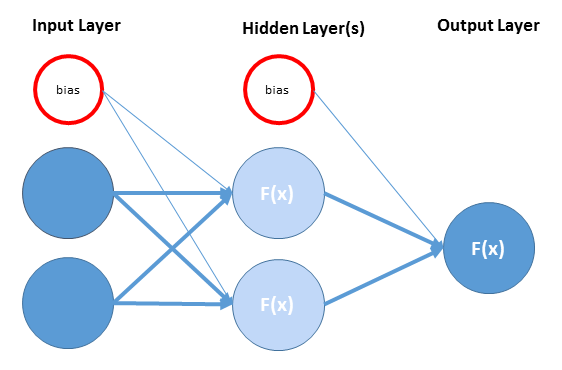
\includegraphics[width=1.0\textwidth]{Figures/SimpleANN.png}
\end{figure}

Often a Bias node is introduced to a connected network. The role of the bias unit is to act as an offset\cite{intro_ml}, shifting the activation function along the y-axis. Bias is implemented by default in Keras. There is an option to turn it off, but if it isn't required, a properly trained network will adjust the weights to zero.

As Stathakis observed\cite{hidden_layers}, traditional methods for identification of topology have been based on trial and error. Trial and error can be time-consuming and, without bounds, could delay more pressing research. The minimum required number of nodes in a network with a single hidden layer is usually the number of inputs\cite{Goodfellow_deeplearning}.

Sometimes, researchers have tried to stick to the following rules-of-thumb for their networks\cite{Saurabh_approx}:
\begin{itemize}
\item The number of hidden layer neurons are 2/3 (or 70\% to 90\%) of the size of the input layer. If this is insufficient then the number of hidden layer neurons can be added later on
\item The number of hidden layer neurons should be less than twice of the number of neurons in input layer.
\item The size of the hidden layer neurons is between the input size and the output size.
\end{itemize}

These mentioned approaches tend to lack sophistication, so some modern methods\cite{huang_two_layer} have tried to limit the maximum number of nodes required for a shallow network (two hidden layers), based on the number of outputs and samples presented. They proved that the number of hidden nodes that are enough to learn N samples with negligible error is given by:
\begin{equation}
    2\sqrt{\left(m+2\right)N} \label{eq:max_neurons}
\end{equation}

This can be further broken down into 
\begin{align}
    &1^{st} \text{Layer}: \sqrt{\left(m+2\right)N} + 2\sqrt{N/\left(m+2\right)} \label{eq:first_layer} \\
    &2^{nd} \text{Layer}: m\sqrt{N/\left(m+2\right)} \label{eq:second_layer}
\end{align}

Where m is the number of output neurons. Note that this does not take into consideration the number of inputs.
Other researchers have looked to use genetic algorithms\cite{learning_algorithm}\cite{hidden_layers} to calculate both the number of nodes and which layer to put them in. These approaches are trying to take the guesswork out of designing the topology of the network, which is designed to save researchers time in building and training their networks.

\subsubsection{Connections between nodes}

The nodes of different layers are connected to each other, as seen in Figure \ref{fig:SimpleNetwork}. There are different ways they can be connected, typically:

\begin{itemize}
    \item Dense / Fully connected
    \item Convolutional
    \item Pooling
    \item Normalisation
\end{itemize}

Densely connected layers are the most commonly used. Every input connects to a nodes, adjusted by a weight vector. The activation function is applied to the sum of these\cite{intro_ml}. The activation function can be linear or non-linear.

Convolutional layers are similar to dense layers. They use a similar matrix multiplication method on the input vector, but filters are used to take only a subset of the data\cite{hidden_layers} at a time. The activation function is usually a differentiable non-linear function. The purpose of convolutional layers in a deep feed-forward network is to reduce over-fitting. Convolutional layers assume that the inputs to the network are images. They are often used in alternating sequence with fully connected layers.

As well as convolutional layers, deep networks often contain pooling layers. In these deep networks, consecutive layers are activated by more complex functions, based off a larger number of inputs. A pooling layer effectively consolidates the outputs of a layer, so that the following layers don't need to perform as many operations. All the valid information is still transmitted, but these layers can help speed up training in large and complex networks\cite{hidden_layers}. Pooling layers are also usually used in networks that take images as inputs. They apply a function such as max or average to a group of outputs of a fully connected layer. This is only useful if those outputs are related in some way, such as in an image.

\begin{figure}[H]
\caption{Architecture of a CNN}
\label{fig:Convolutional}
\centering
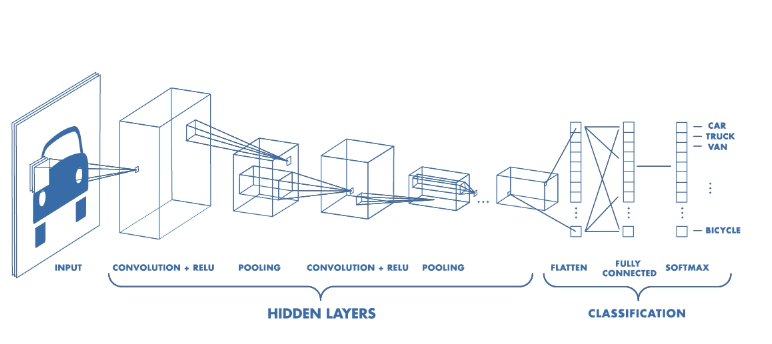
\includegraphics[width=1.0\textwidth]{Figures/convolutional.png}
\source{Medium\cite{conv_nn}}
\end{figure}

There are two main types of normalisation layers. Firstly, they can be used before the input layer for feature scaling\cite{LeCun_backprop}. Secondly, they can be used throughout the network to perform batch normalisation at hidden layers, if a network requires it.

As the inputs to the neural networks in this study are not images, convolutional and pooling layers have not been used. Fully connected and normalisation layers have both been used.

\subsubsection{Activation Functions}

The activation functions at each node should be differentiable semi-linear functions\cite{Rumelhart_error_propagation}. A semi-linear function is required to stop the system collapsing into a single layer linear function\cite{understand_ml}. The function must also be differentiable so that the system can efficiently update the weights through back-propagation of the errors through the network\cite{Rumelhart_error_propagation}. Some examples of common activation functions are sigmoid (Figure~\ref{fig:Sigmoid}), hyperbolic tangent (Tanh: Figure~\ref{fig:Tanh}), Softmax (Figure~\ref{fig:Softmax}) and rectified linear units (ReLU: Figure~\ref{fig:ReLU}).

Because of the way the sigmoid function forces scores to either zero or one, it is commonly used for classification problems. Tanh works in a similar way, and mathematically, Tanh is just a scaled version of sigmoid.

\begin{figure}[H]
\caption{Sigmoid Function}
\label{fig:Sigmoid}
\centering
\begin{equation}
A(x)=\frac{1}{1+e^{-x}}
\end{equation}
\begin{equation}
A'(x)=A(x)(1-A(x))
\end{equation}
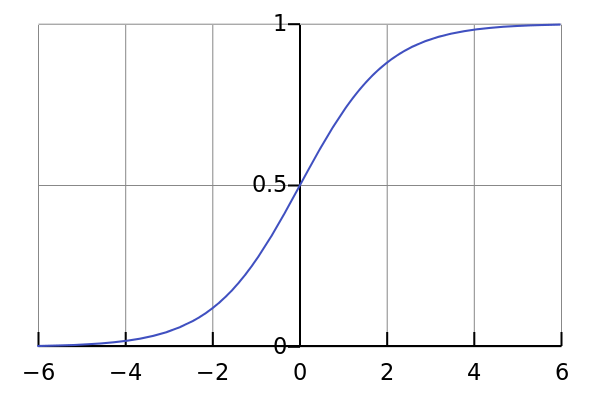
\includegraphics[width=0.6\textwidth]{Figures/Sigmoid2.png}
\source{Medium\cite{activ}}
\end{figure}

\begin{figure}[H]
\caption{Tanh Function}
\label{fig:Tanh}
\centering
\begin{equation}
A(x)=\frac{2}{1+e^{-2x}}-1
\end{equation}
\begin{equation}
A'(x)=1-A(x)^{2}
\end{equation}
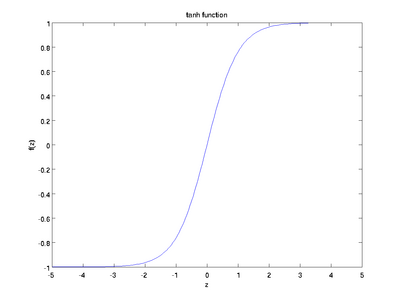
\includegraphics[width=0.6\textwidth]{Figures/Tanh.png}
\source{Medium\cite{activ}}
\end{figure}

Softmax function is also commonly used in classification problems, but usually when there are more than two possible classifications. This is known as multi-classification\cite{intro_ml}. Softmax is used in these cases because the sum of all probabilities will be equal to one, ensuring the outputs are classified distinctly.

\begin{figure}[H]
\caption{Softmax Function}
\label{fig:Softmax}
\centering
\begin{equation}
    A(x)_j = \displaystyle\frac{e^{x_j}}{\displaystyle\sum_{k=1}^{K} e^{x_k}} \text{for}~j = 1, ... , K
\end{equation}
\begin{equation}
    \frac{\partial}{\partial w_i }\sigma(j)=\sigma(j)\left(\delta _{ij}-\sigma(i) \right )x
\end{equation}
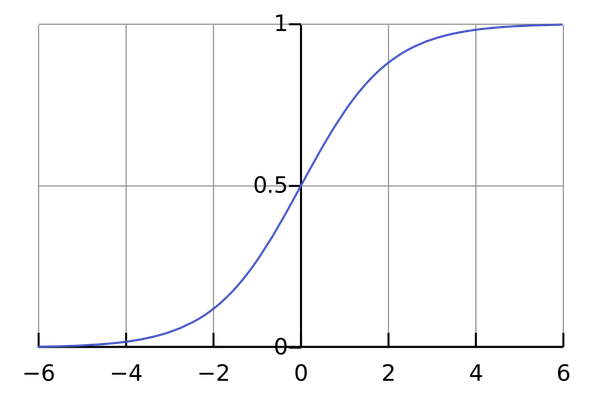
\includegraphics[width=0.6\textwidth]{Figures/Softmax.png}
\source{Introduction to Machine Learning\cite{intro_ml}}
\end{figure}

Where $x$ is an input in the vector $K$,  $j$ is the index of the input unit in $K$, and i is the index of the corresponding output unit. 

There are a number of issues with using these three as activation functions for hidden layers, such as the vanishing gradient problem\cite{LeCun_backprop} where the system stops learning if the gradient becomes too small. This is why, typically, ReLU is used as the activation function for hidden layers. It has also been shown\cite{Krizhevsky_neural} to be much faster in training many classification problems. However because the outputs of our classification problem are binary, ReLU is not appropriate for the output layer\cite{Rumelhart_error_propagation}.

\begin{figure}[H]
\caption{ReLU Function}
\label{fig:ReLU}
\centering
\begin{equation}
A(x)=max(0,x)
\end{equation}
\begin{equation}
A'(x)=1 \text{for} x>1, 0 \text{for} x<=0
\end{equation}
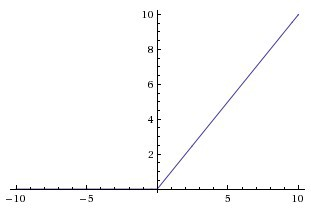
\includegraphics[width=0.6\textwidth]{Figures/ReLU.jpg}
\source{Data Science\cite{diff_activ}}
\end{figure}

From Figure \ref{fig:ReLU} the ReLU activation function returns zero for all negative values. Because the scale of these negative values can be important, especially for inverse relationships\cite{LeCun_backprop} a modified version of ReLU called Leaky ReLU is often used.

In leaky ReLU, the negative values are used, but scaled by a number $\alpha$. $\alpha$ is always smaller than one. It can be fixed, or varied during training. When $\alpha$ is randomly adjusted during training, it can help to avoid over fitting in deep networks\cite{fast_learning}.

\begin{figure}[H]
\caption{Leaky ReLU Function}
\label{fig:Leaky ReLU}
\centering
\begin{equation}
A(x)=\alpha x \text{ for } x<0, x \text{ for } x >=0
\end{equation}
\begin{equation}
A'(x)=1 \text{ for } x>1, \alpha \text{ for } x<=0
\end{equation}
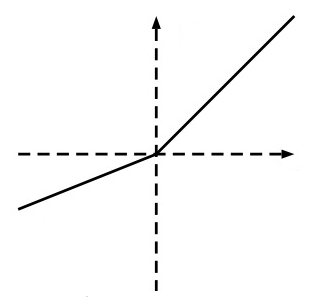
\includegraphics[width=0.6\textwidth]{Figures/LeakyReLU.png}
\source{Data Science\cite{activ}}
\end{figure}

\subsection{Training}

\subsubsection{Normalisation of inputs/outputs}\label{normalisation}

Before training a neural network, it is important to normalise the inputs and outputs. This will make it easier for the network to adjust the weights, and eventually make predictions\cite{Caudill_nn_primer}. Common normalisation techniques in neural networks are:

\begin{enumerate}
    \item Constant normalisation
    \item Min-Max normalisation
    \item Z-score normalisation
    \item Binary encoding
    \item Manhattan encoding
\end{enumerate}

Constant normalisation simply scales the input by a common divisor
\begin{equation}
z=\frac{x}{c}
\end{equation}

Min-Max normalisation forces all values to be within a certain range such as [0,1] or [-1,1]
\begin{equation}
z=\frac{x-min(x)}{[max(x)-min(x)]}
\end{equation}

Z-score normalisation assumes the input is normally distributed and uses the number of standard deviations from the mean as the input. This has the advantage of producing a mean of zero for the input, which LeCun et al.proved to improve convergence of weights\cite{LeCun_backprop} when training a neural network.
\begin{equation}
z=\frac{x_i-\mu}{\sigma}
\end{equation}

Binary encoding is common in neural networks. It is used in classification problems to produce a numeric representation of categories. For example True=1, False=0 or Boys=+1, Girls=-1.

Manhattan encoding is another example of representing classifications\cite{intro_ml}. Typically, 0s and 1s are used in a sequence to represent the classes. For example:
\begin{align*}
    \text{Hong Kong}&=[\;1\;0\;0\;0\;] \\
    \text{Japan}&=[\;0\;1\;0\;0\;] \\
    \text{South Korea}&=[\;0\;0\;1\;0\;] \\
    \text{Taiwan}&=[\;0\;0\;0\;1\;] \\
\end{align*}

This data pre-processing needs to be done before training to give the algorithms a better chance of finding the appropriate weights for a general solution.

\subsubsection{Network Hyper-parameters}\label{subsubsec:hyperparams}

In training a neural network, there are various hyper-parameters that need to be specified for the optimisation algorithm. Many of these parameters come from the generalised delta rule proposed by Rumelhart et al. in 1986\cite{Rumelhart_error_propagation}:
\begin{equation}
    \Delta w_{ij}(n+1)=\eta (\delta _{pj}o_{pi})+\alpha\Delta w_{ji}(n)
\end{equation}

where $\Delta w_{ij}$ is the change to be made to the weight from the $i$th to the $j$th unit following presentation of pattern $p$, $\delta_{pj}$ is the difference between the target input and the actual pattern produced for the $j$th component of the output pattern for pattern ~$p$, the subscript $n$ indexes the presentation number, $\eta$ is the learning rate, $o_{pj}$ is the $j$th element of the actual output pattern produced by the presentation of input pattern $p$, and $\alpha$ is a constant which determines the effect of past weight changes on the current direction of movement in weight space, also known as momentum.

Essentially, what this equation means, is that when a pattern is run through the current network, the result is compared with the target. Then the algorithm works its way back through the network, adjusting the weights on each connection by the difference of the target and observed patterns in proportion to the gradient of the activation function. This adjustment is modified by the learning rate. Also, because of the tendency of a system to fluctuate around the optimum, a momentum term is often included\cite{Rumelhart_error_propagation}. When used, momentum is usually from 0.5 to 0.9, and is it called Momentum Back Propagation (MoBP).

Sometimes, instead of using a momentum term, the learning rate can be decayed\cite{LeCun_backprop}. This will also help avoid the issue of fluctuation as the system will fluctuate less and less with further iterations. This is known as a Variable Learning Rate Back Propagation (VLBP).

When training a network, a variety of learning rates need to be tried. Common best practise is to narrow the search range through 

\begin{equation}
    lr_n = s g^{-n}
\end{equation}

where $lr$ is the learning rate, $s$ is the first learning rate, n is the iteration number, and g is the growth constant, typically 10\cite{Goodfellow_deeplearning}. After a range has been established, smaller a smaller space can be explored with a similarly methodical approach.

\subsubsection{Weights Initialisation}\label{subsec:weights}

To ensure training takes place, it is important to initialise the weights matrix. Rumelhart et al.\cite{Rumelhart_error_propagation} found that training would not occur if weights started at zero and chose random weights close to zero. If all weights are equal initially, every node will calculate the exact same signal. In order to break this symmetry, Hirose et al.\cite{Hirose_backprop} found that random weights limited to certain ranges would not converge:

\begin {table}[H]
\caption{Non-convergence according to Hirose et al.} \label{tab:initial_weights}
\begin{center}
    \begin{tabu}{||c c||} 
        \hline
        \rowfont[c]{\bfseries} Range of weights, ± & Percentage non-convergence  \\
        \hline\hline
        0.05 & 100 \\ \hline
        0.25 & 10 \\ \hline
        0.5 & 0 \\ \hline
        1 & 0 \\ \hline
        1.5 & 20 \\ \hline
        2.5 & 30 \\ \hline
        5 & 50 \\ \hline
    \end{tabu}
\source{Hirose et al.\cite{Hirose_backprop}}
\end{center}
\end{table}

LeCun et al.\cite{LeCun_backprop} furthered this research, suggesting that weights normalised around zero is appropriate. They proposed the range be based on the number of inputs to the layer:

\begin{equation}
    W_{ij} \sim U \left [  - \frac{1}{\sqrt n} , \frac{1}{\sqrt n}  \right ] \label{eqn:lecun1}
\end{equation}

where $W$ is the list of weights vectors, $U[-a, a]$ is the uniform distribution in the interval $(−a, a)$ and $n$ is the size of the previous layer (the number of columns of $W$).

The variance of weights in this case is:

\begin{equation}
    n Var[W] = \frac{1}{3}
\end{equation}

Which means that the variance of the back-propagated gradient is dependent on the layer. It follows that the gradient decreases with n, which increases the chance of the vanishing gradient problem with deeper neural networks\cite{Glorot_difficulties}. Glorot et al.suggested an alternative initialization procedure:

\begin{equation}
    W_{ij} \sim U \left [  - \frac{\sqrt{6}}{\sqrt{n_j + n_{j+1}}}, \frac{\sqrt{6}}{\sqrt{n_j + n_{j+1}}} \right ]    \label{eqn:glorot2}
\end{equation}

which uses the size of the current and following layer instead of the preceding layer. They proposed it maintained both activation variances and back-propagated variances. They called this normalized initialization and it has become the standard default in most neural network libraries such as Keras\cite{chollet2015keras}.

Further to this, to avoid the off chance of landing in a local minimum, it is best practice to run the same training parameters will different initial weights\cite{LeCun_backprop}.

% gradient descent vs ADAM or other optimisers

\subsubsection{Loss functions}\label{subsubsec:loss_func}

The loss function is what a system is trying to minimise overall, and is the judge of how effectively the network is trained. Loss functions typically fall into one of two categories, Regressive loss functions or Classification loss functions\cite{understand_ml}. The type of loss function selected, depends on the outputs required, and on the type of algorithm utilised.

Regressive loss functions are typically used when the target variable is continuous\cite{Nielsen_neuralnetworks}. An example of this is predicting a student's exam scores based on the number of hours studied and the number of hours slept. The most common one is mean squared error (MSE). Absolute error and smooth absolute error are commonly used as well. Mean squared error is calculated by:

\begin{equation}
    g\left ( y, \hat{y} \right )=\frac{1}{n}\sum{\left ( y_i - \hat{y}_i \right )^{2}}
\end{equation}

where $\hat{y}$ and $y$ represent the predicted and target values respectively. It penalises the distance between the predicted and target values.

When the target is a discrete value, classification loss functions are typically used\cite{Goodfellow_deeplearning}. The prediction represents the probability of that classification being true. Some common algorithms are:

\begin{enumerate}
    \item Binary Cross Entropy 
    \item Negative Log Likelihood
    \item Margin Classifier
    \item Soft Margin Classifier
\end{enumerate}

Binary Cross Entropy is the most common loss function for binary classification problems. It measures the divergence between two probability distributions. Binary Cross Entropy is calculated as:

\begin{equation}
    H_{{y}'}(y):=-\sum_{i}{y}'_i\log{y_i}
\end{equation}

where $y_i$ and ${y}'_i$ represent the predicted and target for class $i$, respectively. In the case of binary classification problems, the difference between the predicted probability and value representing the target classification.

Cross entropy is preferred to MSE for classification problems because it is more effective when trying to force the predictions to a distinct value\cite{Caudill_nn_primer}. With MSE, the weight adjustment factor gets smaller, as weights converge, but with cross entropy, the weight changes don't decrease.

\subsubsection{Model Fitting vs Over-fitting } \label{subsubsec:fitting}

When training a neural network, the intention is not to get 100\% accuracy on the training set, but to ensure the network is trained well enough generally to perform well on out-of-sample sets as well\cite{intro_ml}. When a system performs well on the training set, but poorly on the test set, this is known as over-fitting.

The difference between the model's predictions and the target, as calculated by the loss function, is called bias. The sensitivity of a model to small changes in the training set is called variance. High bias means the model has not yet been fully trained while high variance could mean the model has been over-fit.

\begin{figure}[H]
\caption{Bias vs Variance}
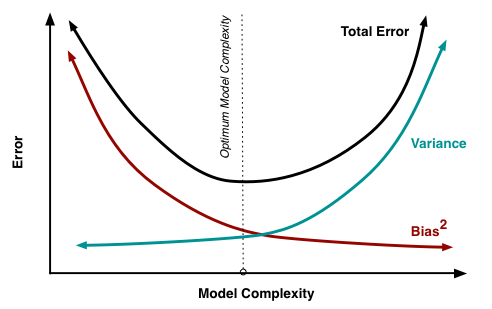
\includegraphics[width=0.9\textwidth]{Figures/biasvariance.png}
\source{Overfitting and Underfitting\cite{over_under}}
\end{figure}

There are various methods employed to avoid over-fitting, such as dropout or early stopping.
% regularisation, cross-validation, batch normalisation

Dropout refers to a practise in training a deep neural network, where some neurons are randomly selected to be ignored during a training run\cite{Goodfellow_deeplearning}. By dropping neurons during training, it reduces the co-dependency formed between the nodes and forces redundancy in the network\cite{Srivastava_dropout}. When training is complete, the 'dropped' nodes are added back for testing. According to Srivastava et al. this gives major improvements over other regularization methods because it is effectively averaging the predictions of all the thinned networks\cite{Srivastava_dropout}.

\begin{figure}[H]
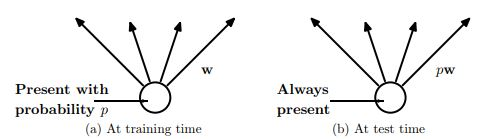
\includegraphics[width=0.9\textwidth]{Figures/Dropout.JPG}
\end{figure}

Nodes, and their connections are dropped based on a probability during training stages, but always present during testing. Whilst this is now a widely accepted practise for deep neural networks, for shallow neural networks, it is less effective\cite{Srivastava_dropout}.

For shallow networks, it is common to stop the training as soon as it has reached a certain level of accuracy, or after a certain number of epochs (training runs)\cite{Caudill_nn_primer}. This will have the effect of preventing over-fitting, as the network doesn't have the chance to perfectly fit the training set.

In early stopping, the data is typically divided into three sets\cite{girosi_neural}:
\begin{itemize}
    \item Training
    \item Validation
    \item Testing
\end{itemize}{}

The training set is the largest, it is usually 60\% to 70\% of total data. This is the set the model uses to adjust weights during stochastic gradient descent. The validation set is also used in testing, but it is used by the early stopping algorithm to check the effectiveness of training. If training has stagnated, and the model hasn't improved for a set number of iterations, the training is stopped early\cite{chollet2015keras}. The validation set needs to be at least 10\% of the testing set and is usually up to 20\%.

The testing set is used for the evaluation of the model. It was not used in testing and the model hasn't seen it before. This is the true test of the effectiveness of the model\cite{Prechelt97earlystopping}. As well as checking the loss function, the model can make predictions and check them against the expected values of the testing set.

As discussed by Ripley \cite{ripley2007pattern}, it is best practice to randomly select the the training, validation and testing sets from the total data, but it is important to ensure that the distribution is similar.

\subsection{Interpreting the output}

When the output produced by the neural network is a probability, between 0 and 1, the system needs a way of attributing this to a discrete classification. This requires a threshold level to be calculated.

The most common way of attributing this probability to a signal is through a receiver operating characteristics (ROC) graph\cite{Fawcett_threshold}. ROC graphs is a technique for organising, visualising and selecting classifiers based on their performance.

\begin{figure}[H]
\caption{Confusion matrix and commonly derived performance metrics}
\label{fig:ConfusionMatrix}
\centering
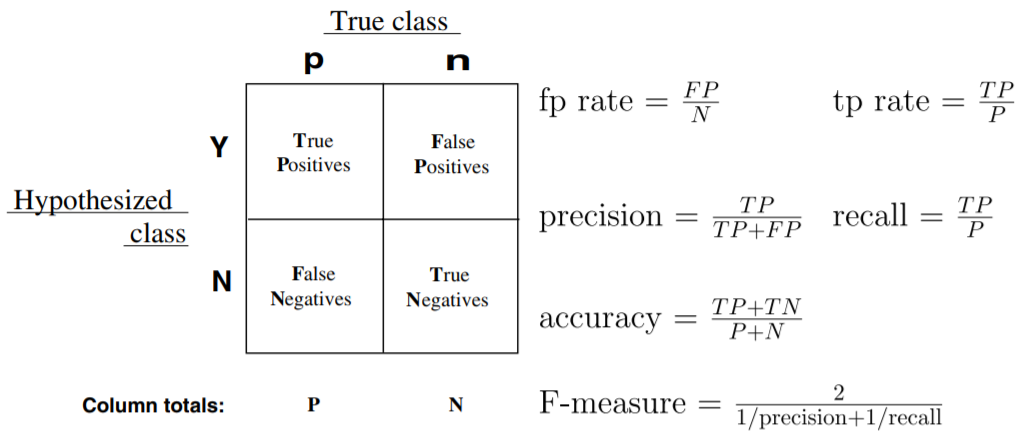
\includegraphics[width=1.0\textwidth]{Figures/ConfusionMatrix.png}
\source{Fawcett\cite{Fawcett_threshold}}
\end{figure}

Where fp rate is the false positive rate (type 1 errors) and tp rate is the true positive rate. Another common term is specificity, which is 1-fp rate. The precision is also often called the positive predictive value.

ROC graphs show the trade-off between the accurate predictions for true positives, and the type one errors potentially made. In an ROC graph, the fp rate from figure~\ref{fig:ConfusionMatrix} is plotted on the X axis and the tp rate is plotted on the Y axis. Points in the top left hand corner of the graph are the most desirable.

To compare points on this graph that are not directly related, area under curve (AUC) is calculated\cite{Guerriere_NN}. Because the axis are both proportions from 0 to 1, this calculated area will always be less than 1. The threshold that gives the highest AUC value according to equation \ref{eqn:auc} is the optimal threshold.

\begin{equation}\label{eqn:auc}
    AUC = \text{tp rate} * (1-\text{fp rate})
\end{equation}

This method of evaluation is commonly used in medical analysis, and other studies where the incidence rate of positives is expected to be low. However, this analysis required that a recommendation or decision be made. In financial services, unknown is also acceptable\cite{efficient_markets}.

This adjusts the calculation for tp to:

\begin{equation}\label{eqn:tp_adj}
    \text{tp rate} = \frac{TP}{P+UD}
\end{equation}

Where UD is the uncategorised responses. When this is calculated, the ROC can still be generated and the AUC can be calculated and compared.

\pagebreak
\section{Event Studies in Financial Markets}

\subsection{Asset classes}

An asset class is a term used to describe a group of securities with similar investment characteristics. These characteristics usually include risk profile, transaction costs, expected returns, and government regulations\cite{ross_corp}. The major asset classes are:

\begin{itemize}
    \item Equities
    \item Fixed Income
    \item Cash/FX
    \item Alternative Investments
\end{itemize}

The most popular asset class with retail investors is equities. Equities typically refers to common stock in a company listed on an exchange. But can also refer to preference shares, and exchange-traded funds (ETFs) and indices based on these. These instruments are only available to trade during specified market hours and usually not on weekends. Prices of these typically fluctuate more than fixed income and cash.

The other largest asset class for direct investment is fixed income. Fixed income refers to debt instruments issued by corporations, governments and related entities. It includes zero-coupon bonds and short-term money market instruments. These are typically traded over-the-counter (OTC) through an intermediary rather than on an exchange. Because bonds have seniority in the case of default and have a maturity date, they are usually considered a less risky investment than equities\cite{ross_corp}.

Cash includes all cash holdings which is considered to be zero-risk other than the inherent foreign exchange risk. Unlike other asset classes, FX markets are open 24 hours, 7 days a week. The foreign exchange market is by far the most liquid asset class by daily value traded\cite{ross_corp}.

Alternative investments is a large class, with many different sub-sections. These include commodities, direct real estate, art, private equity and more recently, crypto-currencies. Other than commodities, where secondary markets with regular trading contracts have been established, most alternative investments are considered illiquid, and not suitable for short-term trades\cite{efficient_markets}.

Most Equities, Fixed Income and FX instruments can be sold short directly\cite{ross_corp}. However, Market makers have established derivative markets on all of these asset classes including commodities. This allows investors to take positions on both the long and short sides of a trade\cite{agg_react} if they're not able to short the instrument directly.

Other than the commodities in the sections above, most of the instruments in each asset class belong to some kind of index. These indices are considered less risky to trade than single stocks because much of the company specific risk is diversified away.

Another option to trading a single instrument long or short, is a pair trade. A pair trade is when the investor goes long in one instrument, and short in another\cite{ross_corp}. The purpose of this is to gain exposure to some specific pricing differential while hedging some of the market risk inherent in a one-sided trade.

When trading financial instruments it is important to take into consideration transaction costs. The liquidity analysis required for these short term instruments is beyond the scope of this paper, but is important to note that this could negate any potential profits made from the trades.

\subsection{Event Study Methodology}

Testing for potential sources of alpha in financial markets is performed by both academics and market practitioners. This is especially true since Burton's work on random returns in 1973\cite{burton_random_walk}. With the power of modern computers, many researchers are using unsupervised learning. However, Keogh and Kasetty\cite{data_mining_Keogh} tested over 20 different data mining algorithms on over 50 different data sets with a view to verifying their utility. Their conclusion was that the data mining community needs to reduce the occurrence of implementation bias in their experiments and introduce objective benchmarks to verify algorithms.

Zhang and Zhou\cite{golden_nuggets} also examined the application of various data mining techniques to the finance industry. Specifically, they looked at Stock market predictions, portfolio management, bankruptcy prediction, foreign exchange markets, and fraud detection. They highlighted that the selection of appropriate inputs and algorithms, as well as model refinement and assessment are key components of event studies. Also, although neural network modelling is the most widely used method in data mining applications in finance, the optimal design of neural networks for various financial engineering problems remains open. At this stage they were not able to provide suggestions for appropriate algorithms and neural networks.

Because of these limitations, this report focuses on more traditional event study analysis using hypothesis testing. In more traditional event study analysis, first boundaries for the testing space must be established. Then, the space should be methodically searched for the results\cite{data_mining_Keogh}.

\subsection{Hypothesis testing}\label{subsec:hyp_test}

Hypothesis testing is a statistical approach to decision making.  Hypothesis testing first makes a tentative assumption about the expected results, and then uses logical or empirical tests to produce a statistical probability or confidence that the assumption is true or false.
%A hypothesis, as defined by the Merriam Webster dictionary is, \textit{"a tentative assumption made in order to draw out and test its logical or empirical consequences"}\cite{MerriamWebster2009}.

To conduct a hypothesis test, there are six main steps to follow\cite{black_stats}:
\begin{enumerate}
    \item Define Alternate Hypothesis and Null Hypothesis
    \item Decide on level of significance/confidence interval
    \item Calculate t-stat
    \item calculate p-value
    \item Make a decision on the null hypothesis
    \item Summarise conclusions based on decision
\end{enumerate}

A null hypothesis is the hypothesis assumed to be true, unless proven otherwise. The Alternate hypothesis is what the research is trying to prove. The alternate hypothesis is either:
\begin{itemize}
    \item The tested parameter is not equal to a certain value (a two sided test)
    \item The tested parameter is less than a certain value (left-tailed test)
    \item The tested parameter is greater than a certain value (right-tailed test)
\end{itemize}

The most commonly used significance level for event studies involving financial returns analysis is 95\%, which is approximately 2 standard deviations away from the mean in a normal distribution.

Because this work will involve forecasts, and the population's standard deviation is not known, the most appropriate statistic is the t-statistic\cite{black_stats}. The t-stat is based on the sample standard deviation:

\begin{align}\label{eq:tstat}
    t &= \sqrt{n}\frac{\Bar{x}-\mu}{s} \\
    df &= n-1 \nonumber
\end{align}

Where $t$ is the statistic calculated, $\Bar{x}$ is the sample mean, $s$ is the sample standard deviation and n is the number of observations. df refers to degrees of freedom. The formula in equation~\ref{eq:tstat} is for tests of a single population against a constant number, often zero. To test if the mean of two populations is significantly different, the formula is adjusted to include the distribution of the second population.

\begin{align}\label{eq:tstat_two}
    t&=\frac{\bar{Y_1}-\bar{Y_2}}{\sqrt{s_{1}^{2}/N_1+s_{2}^{2}/N_2}}
\end{align}

The p-value is calculated based on this statistic, and represents the probability of this being significant. P-values are compared to $\alpha$, which is calculated by:
\begin{equation*}
    \alpha = 1 - \text{Significance Level}
\end{equation*}

If the p-value is less than alpha, the null hypothesis is rejected. If the p-value is greater, the null hypothesis cannot be rejected. After the null hypothesis is rejected or not, the conclusions about the test can be discussed.

Because these are based on statistics, there is also a probability of error\cite{hypothesis}. There are two types of error; type 1 and type 2 errors. Type one error is false positives, where the test rejected a null hypothesis which is actually true. Type two error is a false negative, where the test did not reject the null hypothesis, when it is true.

Jegadeesh and Knaub\cite{jegadeesh_returns}\cite{knaub_hypothesis} both found evidence of excess returns in the stock markets using these methods. However, it should be noted, that they were both using end of day market data, unlike this report which looks at intra-day.

When performing any hypothesis test, it's also important to understand the assumptions behind the statistics\cite{black_stats}. When performing a t-test there are four main assumptions:

\begin{enumerate}
    \item The data is collected from a randomly selected and representative portion of the population.
    \item The data collected follows a continuous, and not discrete scale.
    \item The sample is a reasonably large size and follows a normal distribution.
    \item The variance of the sample is approximately equal to other samples from the same population.
\end{enumerate}

In order to have confidence of these holding true, the normality of a sample can be tested by measuring the skewness and kurtosis of the sample\cite{hypothesis}. These can be plotted and tested with regression analysis. Along with standard deviation, skewness and kurtosis explain the shape of the distribution. To test the assumption of normal distribution, skewness should be within $\pm$0.5 and kurtosis should be within range of $\pm$2.

To test that the sample is a reasonably large size, the below formula can be used:

\begin{equation} \label{eq:minpop}
    \text{Minimum Population} = \frac{Z^2 * \sigma (1- \sigma)}{me^2}
\end{equation}

Where $Z$ is the z-score of the confidence interval, $\sigma$ is the standard deviation of the sample, and $me$ is the margin of error accepted for the study\cite{black_stats}.

For a two-sample t-test, the above assumptions of normality also must hold true for both samples. Further to this, the standard deviations must be similar. This is tested by a F-test:

\begin{equation} \label{eq:fstat}
    F = \left( s^{2}_{1}/s^{2}_{2} \right)
\end{equation}

Where $F$ is taken from the critical value of the F distribution. For a two tailed F-test, it passes if $F$ is outside of the bounds calculated by the significance level chosen:

\begin{equation} \label{eq:fdist}
    F < F_{1 - \alpha/2,N_1 - 1,N_2 - 1}  \\
    or \nonumber\\
    F > F_{\alpha/2,N_1 - 1,N_2 - 1} \nonumber\\
\end{equation}

Even if a t-stat suggests the null hypothesis should be rejected, we cannot draw that conclusion if any of the assumptions are violated\cite{knaub_hypothesis}.

As well as tests that the returns are significantly different from zero, investors want to only invest where there is a reasonable risk/reward ratio. For analysing returns, the most common ratio is the sharpe ratio\cite{perf_eval}. This was first proposed by William Sharpe in 1966\cite{sharpe_perf} and describes returns in proportion to their risk.

\begin{equation}
    \text{Sharpe} = \frac{\Bar{r_p} - r_f}{\sigma _p}
\end{equation}

Where $r_p$ is the mean portfolio return, $r_f$ is the risk-free rate and $\sigma _p$ is the standard deviation of portfolio returns. Sharpe ratio greater than 1 is considered a "good" strategy\cite{ross_corp}. There are other measures such as Jensen's measure and Treynor ratio which are more equity specific and not applicable to other asset classes. Sharpe is widely used because it adjusts for a security's cost of capital through the risk free rate and can be applied to any publicly traded asset.

%Background:
%The goal is for your the contents of the literature review to be thorough with respect to the important statistical literature related to the problem.
% only want to cite publications that are related to your research.
%²  want to discuss how the cited literature is related to your research. That is,  want to refer to published research to motivate the originality and %relevance of your research.

 % Background Theory 

\chapter{Twitter filtering and classification}

\section{Downloading Tweets}

Downloading historical tweets through the official Twitter API is not possible without paying for the enterprise edition\cite{Twitter_api}. Also, most third party tools to download historical tweets are expensive to use. Fortunately there is one free library built for this, and this paper utilised GetOldTweets-python by Jefferson-Henrique\cite{getoldtweets}. Henrique automates Twitter's in-browser search function's scroll loader through JSON calls. The disadvantage of this method is that it only does one handle at a time.

This paper has limited the news agencies to fifteen of the major world-wide English agencies. All have been active on Twitter since at least 2011. The details of these are in Table~\ref{tab:news_agencies}.

These fifteen news agencies tweeted a total of 387,063 tweets in the 18 months from 1st January 2017 to 30th June 2018. For consistency, this paper will refer to them collectively as news tweets, and when referring to specific tweets, will use the Twitter handle.

In the same time period, there were 470 tweets signalling earthquakes from the @USGSted Twitter handle, the official U.S. Geological Survey earthquake alerts. These will be called USGS tweets.

\begin {table}[H]
\caption{News Agencies Used} \label{tab:news_agencies} 
\begin{center}
    \begin{tabu}{||l l l||} 
        \hline
        \rowfont[c]{\bfseries} Agency & Handle & Since \\
        \hline\hline
        Agence France-Presse & @AFP & 2011-09-01 \\
        \hline
        Asian News International & @ANI & 2011-08-01 \\
        \hline
        Associated Press & @AssociatedPress & 2009-06-01 \\
        \hline
        Australian Associated Press & @AAPNewswire & 2011-01-01 \\
        \hline
        Bloomberg & @Bloomberg & 2010-01-01 \\
        \hline
        Canadian Press & @CdnPress & 2009-05-01 \\
        \hline
        Catalan News & @catalannews & 2010-01-01 \\
        \hline
        CNN News & @CNN & 2007-02-01 \\
        \hline
        Dow Jones & @DowJones & 2010-06-01 \\
        \hline
        EFE Noticias & @efenoticias & 2010-01-01 \\
        \hline
        Press Association & @PA & 2009-02-01 \\
        \hline
        Press Trust of India & @PTI\_News & 2011-02-01 \\
        \hline
        Reuters & @Reuters & 2007-03-01 \\
        \hline
        United Press International & @UPI & 2008-10-01 \\
        \hline
    \end{tabu}
\end{center}
\source{Bloomberg\cite{bloomberg}}
\end{table}

\pagebreak
\section{USGS Tweets}

The USGS tweets are in a standardised format. This makes extracting the location, magnitude and time-stamp of the earthquake a simple exercise in string comprehension, as per the code in Listing~\ref{lst:extracting}:

\begin{figure}[H]
\caption{Tweet from USGS on May 9}  \label{fig:USGSTed} 
\centering

\includegraphics[width=0.8\textwidth]{Figures/USGSTed_May9.PNG}
\source{\url{https://Twitter.com/USGSted}}
\end{figure}

The geopy library takes a location string and places it on the globe\cite{geopy}. There are a variety of geocoders to chose from such as Bing Maps, Nominatim and Google. GoogleV3 is the same database driving google maps and provides accurate latitude and longitude, based on a location string entered.

\begin{lstlisting}[caption={Extracting data from standardised USGS tweets}, captionpos=t, label={lst:extracting}]

import numpy as np
from datetime import datetime as dt
from geopy.geocoders import GoogleV3
geolocator = GoogleV3(api_key=private_api_key)
class TweetText():
    #extract magnitude, location and time from standardised tweets by USGSted
    # "Prelim M6.5 earthquake Java, Indonesia Dec-15 16:47 UTC, updates https:// go.usa.gov/xnnuP , 398 #gempa tweets/min"
    def __init__(self, text, date):
        # find the dash from the end of the string
        dash_loc = text[::-1].find('-')
        self.region = text[23:-(dash_loc+4)].strip()
        try:
            location = geolocator.geocode(self.region)
            self.coordinates = (location.latitude, location.longitude)
        except:
            self.coordinates = np.NaN
        self.magnitude = text[8:12].strip()
        self.timestamp = dt.strptime(date[0:4]+'-'+text[-(dash_loc+4):-(dash_loc-8)].strip(), '%Y-%b-%d %H:%M')
        self.details = [self.magnitude, self.region, self.coordinates, self.timestamp]
\end{lstlisting}

The time of earthquake given by USGS is in Coordinated Universal Time (UTC). However, the time-stamp for tweets downloaded from the Twitter website using GetOldTweets is the user's local time. Because, in this case, that is Hong Kong, these times had to be converted to UTC. After conversion, all times in this paper are in 24-hour UTC unless otherwise specified.

The 470 USGS tweets were all processed and cleaned in this way.

\pagebreak
\section{Pre-processing}

\subsection{Network Inputs}

The purpose of this system is to test if a tweet is referring to the same earthquake event as one specified by a USGS tweet. To identify these tweets, a combination of automated filtering and neural network classification will be used. The purpose of the filtering and classification will be to help reduce the amount of work the neural network has to perform, by reducing the inputs to only those most important to classification.

Given that it's possible for two earthquakes to strike in different parts of the world at a similar time, the first input was based on distance. By comparing distances, it will increase the chance of only selecting relevant tweets.

Given the speed that news can travel, it is important to consider the timeliness of the tweets from news agencies. The second input was based on the difference in time between the USGS tweet and the news tweet.

For financial signals, it's important to be first. So as well as the distance and time differences, whether the same news agency, or any news agency has mentioned the tweet or not was also used. Without these checks, multiple tweets from the same source could be identified as relevant.

In summary, the network inputs chosen were:
\begin{itemize}
    \item Great Circle Distance between the earthquake location and the location mentioned in the news tweet
    \item Time from news tweet to USGS tweet
    \item Whether this particular news agency has reported this earthquake before.
    \item Whether any news agency has reported it before.
\end{itemize}

Across the tweets selected, the first two continuous-scale inputs had a correlation of only 0.165 which indicates that it is not likely to have any redundancy from them. By ensuring the number of inputs is contained to the minimum required for a human to check, the complexity of the model is contained.

\subsection{Data Cleansing and Filtering}

A large part of training a neural network is ensuring the data is clean and in a usable form\cite{LeCun_backprop}. There were five steps to this process:

\begin{enumerate}
    \item Filter the data by keyword
    \item Extract locations from the text, translate to coordinates
    \item Merge USGS tweets DataFrame with News Agency tweets DataFrame
    \item Calculate differences between locations and time-stamps
    \item Filter out news agency tweets which happened before the earthquake, or more than three days after the respective USGS tweet.
\end{enumerate}

After all these steps were complete, the manual coding of the data could begin.

The first step in preparing the news agency tweet data was filtering the tweets which also contained key words related to earthquakes. Merriam Webster dictionary highlighted this list related to earthquakes: [`quake', `earthquake', `magnitude', `earthquake', `Richter', `aftershock', `tremor', `seismic', `epicenter', `epicentre']\cite{MerriamWebster2009}.

This left a list of only 1040 tweets, to use in training the neural network. The vast majority were related to earthquakes, such as ``7.9 earthquake strikes near Papua New Guinea, Solomon Islands http:// upi.com/6484906 pic.Twitter.com/j2NjsjAshF" or ``An earthquake of 6.1 magnitude hit Northern and Central Iran at 3.11 am." Unfortunately, some of the tweets were unrelated: ``A `youthquake' struck 2017 as Oxford Dictionaries' word of the year http:// u.afp.com/4Fgx" and ``If the U.N. sexual abuse crisis has an epicenter, it is the Congo.". These tweets were kept and used in training the network. They were classified as unrelated to any earthquake, and will be used by the system to avoid future possible scenarios.

Next, the Polyglot library was used to do named entity recognition for locations of the earthquake the tweets are referring to\cite{polyglotner}. Polyglot was chosen over other NER libraries because it supports languages other than English. In future work it will be important to source tweets from a more global base. The only entities used in this research were locations, using the `I-LOC' tag, as per Listing~\ref{lst:ner}:

\begin{lstlisting}[caption={Named Entity Extraction with polyglot}, captionpos=t, label={lst:ner}]
import polyglot
from polyglot.text import Text
def get_location(blob):
    text = Text(blob, hint_language_code='en')
    location = ''
    for entity in text.entities:
        if entity.tag == 'I-LOC':
            location+= " ".join(entity) + ', '
    return location

df_quakes['location'] =  df_quakes.text.apply(lambda x: get_location(x))

\end{lstlisting}

The 470 USGS tweets were merged to the 1040 tweets to give a DataFrame with 488,800 rows.  The tweets are all time-stamped for publication date which can be used to calculate the time difference between the USGS tweet and the news tweet.

Using the location coordinates indicated in the news tweets and the USGS tweets, the great circle distance between the two points is calculated. Dyck's implementation of the Haversine formula was used\cite{haversine}.

The penultimate step was using the time differences. The time-stamps were converted in the same way as the USGS tweets then rows were removed where:

\begin{enumerate}
    \item the news tweet came before the earthquake time-stamp in the USGS tweet.
    \item the news tweet was more than three days after the USGS tweet
\end{enumerate}

It is important to include news tweets that came before the USGS tweet to test for any news agencies that might have a source faster than USGS, as long as they were after than the actual earthquake. When this final filtering step was complete, there were 3654 rows.

\subsection{Output Coding}

For training, the related tweets need to be manually classified. In classifying, the focus was on Breaking news. Updates on rescue efforts and death toll numbers were considered unrelated as they are no longer useful for identifying an earthquake has occurred.

Figure~\ref{fig:USGSTed} showed an example of the standardised tweets produced by the USGS. It was tweeted at 10:58 on 2018-05-09, and is referring to an earthquake that occurred 17 minutes previously in the Afghanistan-Tajikistan-Pakistan region. Table~\ref{tab:sample_tweets} shows the filtered news tweets within three days of that USGS tweet. 

The first tweet from @ANI that referred to the earthquake was at 11:13, 15 minutes after the USGS tweet, and 32 minutes after the earthquake hit. A number of tweets around that time were marked as not related because they referred to an earthquake that happened in China on the same day, ten years prior. @AFP made two tweets shortly after the earthquake. One at 11:15, that references USGS as a source. They posted again at 13:30, with a story and link. This was quite a common occurrence in the data set. News agencies would post the headline in an attempt to break the news first, and then write a story around it.

Table~\ref{tab:delayed_coverage} shows the average delay after the USGS tweet to the first relevant news agency tweet.

\begin {table}[H]
\caption{How soon do news agencies cover earthquakes?} \label{tab:delayed_coverage}
\begin{center}
    \begin{tabu}{| l r |} 
        \hline
        Shortest Delay: & 3 mins \\
        Mean Delay & 124 mins \\\
        Median Delay & 35 mins \\
        Longest Delay & 977 mins  \\ \hline
    \end{tabu}
\end{center}
\end{table}

\begin{sidewaystable}[htbp]
    \caption{Tweets tested against USGS May 9$^{th}$ tweet}
    \label{tab:sample_tweets}
    \bigskip
    \centering\small\setlength\tabcolsep{2pt}
        \hspace*{-2cm}\begin{tabular}{ p{4cm} p{2cm} p{16cm} p{3cm} }
            \toprule
            \textbf{Tweet Timestamp} & \textbf{Agency} & \textbf{Tweet Text} & \textbf{Classification} \\
            \midrule
2018-05-09 11:13 &  ANI & Earthquake of magnitude 6.2 hit Afghanistan-Tajikistan-Pakistan region: USGS, light tremors were felt in parts of northern India, including Delhi \& Kashmir. & TRUE \\
2018-05-09 11:15 &  AFP & \#BREAKING Strong 6.2-magnitude earthquake rocks Afghanistan: USGS & TRUE \\
2018-05-09 12:00 &  AFP & VIDEO: As China prepares to mark 10 years since the 7.9-magnitude Sichuan earthquake, around 200 people work to preserve the ruined buildings of Beichuan, a city frozen in time since May 12, 2008 pic.Twitter.com/jFd0Y8AW92 & FALSE \\
2018-05-09 13:30 &  AFP & \#UPDATE A strong 6.2-magnitude earthquake has rocked northern Afghanistan, the US Geological Survey says, creating tremors felt as far away as Pakistan's capital Islamabad and Tajikistan's Dushanbe http://u.afp.com/ox8v pic.Twitter.com/RQtx8L7Kb7 & TRUE \\
2018-05-09 14:11 &  CNN & Hawaii residents could face acid rain after earthquakes and molten lava https://cnn.it/2G03r2G pic.Twitter.com/9SZWwYwPXs & FALSE \\
2018-05-09 17:17 &  UPI & Earthquakes strike Afghanistan, Pakistan https://www.upi.com/Top\_News/US/20 18/05/09/ Earthquakes-strike-Afghanistan-Pakistan/1571525883573/?utm\_source=dlvr.it\&utm\_medium=Twitter & TRUE \\
2018-05-09 18:25 &  CNN & Hawaii residents could face acid rain after earthquakes and molten lava https://cnn.it/2rv69be pic.Twitter.com/7EsLzI6utN & FALSE \\
2018-05-10 05:46 &  CNN & Hawaii residents could face acid rain after earthquakes and molten lava https://cnn.it/2rygcw5 pic.Twitter.com/7rp3vm2S47 & FALSE \\
2018-05-10 06:28 &  AFP & Life among the ruins: Chinese village 10 years after devastating earthquake in Sichuan left 87,000 people dead or missing http://u.afp.com/oxbq Johannes Eisele @johaynz pic.Twitter.com/CENCPfllNP & FALSE \\
2018-05-10 07:52 &  AFP & VIDEO: 'Strong Pig' is a celebrity in China after surviving the devastating Sichuan earthquake a decade ago that left 87,000 people dead or missing pic.Twitter.com/Iap71OHFR5 & FALSE \\
2018-05-10 09:22 &  CNN & Hawaii residents could face acid rain after earthquakes and molten lava https://cnn.it/2KRrm7Z pic.Twitter.com/grKq4ruf3A & FALSE \\
2018-05-10 19:42 &  AFP & VIDEO: The tiny hamlet of Radish Village in China's southwest is one of several in Sichuan province that decided to preserve the destruction as a memorial to the 2008 earthquake pic.Twitter.com/7FwXCEqPQE & FALSE \\
2018-05-11 18:02 &  Reuters & Hawaii residents shaken by quakes, brace for new lava outbreaks https://reut.rs/2rBJ0UG & FALSE \\
2018-05-11 20:16 &  Reuters & Hawaii residents shaken by tremors, brace for new lava outbreaks https://reut.rs/2KS5kSG & FALSE \\
2018-05-12 07:06 &  UPI & On This Day: Sichuan earthquake kills tens of thousands https://www.upi.com/Top\_News/2018/ 05/12/On-This-Day-Sichuan-earthquake-kills-tens-of-thousands/4111526048817/ ?utm\_source=dlvr.it\&utm\_medium=Twitter & FALSE \\
2018-05-12 07:31 &  ANI & An earthquake of magnitude 3.0 on the Richter scale hit Chamba region of \#HimachalPradesh at 9:27 am today & FALSE \\
           \bottomrule
        \end{tabular}
        \source{Twitter }
        \hspace*{-2cm}
\end{sidewaystable}

Of the 3654 records in the training data only 294, or 8\% were coded as relating the news tweet to an earthquake.

\begin{figure}[H]
\centering
 \caption{Tweet Classification Summary}
 \label{fig:classification}
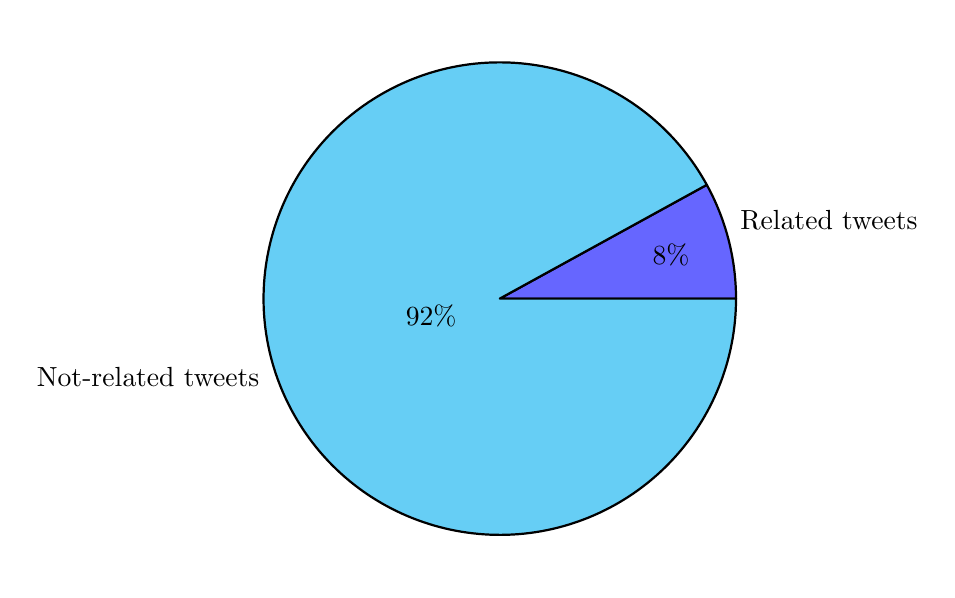
\begin{tikzpicture}
 \pie [rotate = 0]
    {8/ Related tweets,
     92/ Not-related tweets}
\end{tikzpicture}
\end{figure}

\subsection{Dividing the Data Set}

As discussed in Sub-section~\ref{subsubsec:fitting} the data needs to be divided into three sets; training, validation and testing.

75\% of the data set was randomlly selected to be used as training, and 25\% to be used as testing. The next step is to divide the training set into the actual training data and the validation data set. A similar algorithm was used to assign 20\% of the training data to a validation set. The final breakdown can be seen in table~\ref{tab:breakdown}.

\begin {table}[H]
\caption{Data set Breakdown} \label{tab:breakdown}
\begin{center}
    \begin{tabu}{| c c c c | } 
        \hline
        \rowfont[c]{\bfseries} Data Set & Records & \% of Total & \% Related \\
        \hline\hline
        Training Set & 2192 & 60 & 8.0 \\
        Validation Set & 548 & 15 & 7.1 \\
        Testing Set & 914 & 25 & 8.6 \\ \hline
        \textbf{Total} & \textbf{3654} & \textbf{100} & \textbf{8.0}\\ \hline
    \end{tabu}
\end{center}
\end{table}

While running training iterations, this was repeated for each iteration, as well as randomising the initial weights. As mentioned in Sub-section\ref{subsec:weights} Keras automatically randomises the initial weights according to Glorot's algorithm\cite{chollet2015keras}.

\pagebreak
\section{ANN Setup}

There are a large number of freely available machine learning resources for python. This streamlines the model building process. This project utilises a high-level neural network API called Keras\cite{chollet2015keras} running on top of Google's the TensorFlow framework\cite{tensorflow2015-whitepaper}.

\subsection{Normalisation Layer}

Before attempting to train a network with this data, it is important to normalise the inputs, as discussed in Chapter 2's section on normalisation (\ref{normalisation}). For the distance and time inputs, the min-max method was used. All distances were represented as a percentage of the maximum possible distance (half the earth's circumference). All times were converted to seconds, and calculated as a percentage of the seconds in three days: $3 * 24 * 60 * 60 = 259 200$, including the negative values. The tests on whether or not a particular news agency covered an earthquake before was coded from True/False to 1/0.

\subsection{Network Topology Set-up}

As discussed, there are four normalised inputs to the neural network. In all cases for this network, boolean data is represented by 0 for False, and 1 for True.
\begin{itemize}
  \item Great Circle Distance: as a percentage of the earth’s half circumference
  \item Time Lapsed: as a percentage of 3 days
  \item Whether this news agency has reported it: boolean
  \item Whether any news agency has reported it: boolean
\end{itemize}

If any of these fields are not useful in calculating the outputs, their weights will tend towards zero. The output, expected of the neural network is whether or not it is related to the earthquake.

\begin{figure}[H]
\caption{Example of the neural network}
\centering
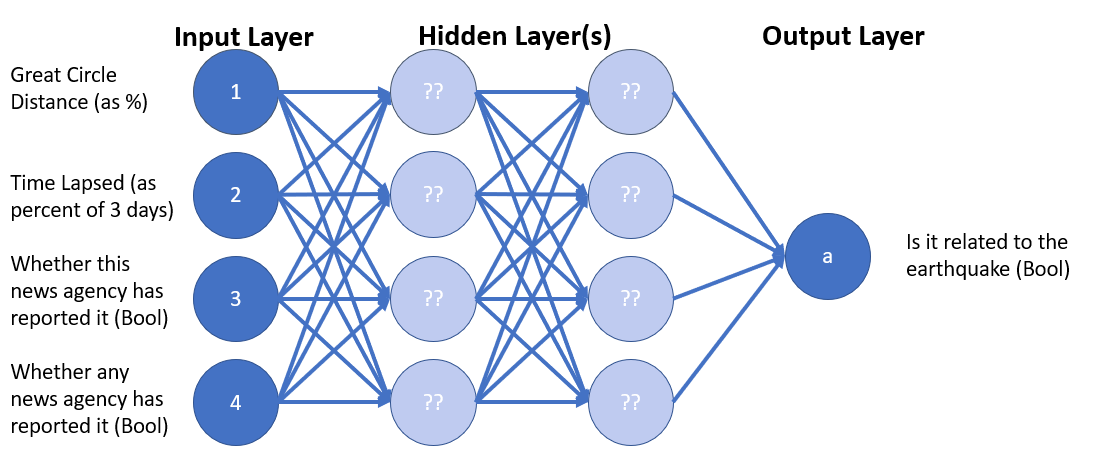
\includegraphics[width=1.0\textwidth]{Figures/SampleNetwork.PNG}
\end{figure}

For such a simple data set, a deep network will likely not be required. Prior research\cite{LeCun_backprop}\cite{Goodfellow_deeplearning}\cite{huang_two_layer} suggests one or two-layers will be sufficient.

Reviewing formulas ~\ref{eq:first_layer} and ~\ref{eq:second_layer} in Chapter 2, the number of outputs, $m$ is 1, the number of training samples, $N$, is 2192.
\begin{align*}
    1^{st} \text{Layer}&= \sqrt{\left(m+2\right)N} + 2\sqrt{N/\left(m+2\right)} \\
    &= \sqrt{\left(1+2\right)2192} + 2\sqrt{2192/\left(1+2\right)} \\
    &= 135 \\
    2^{nd} \text{Layer}&= m\sqrt{N/\left(m+2\right)} \\
    &= 1\sqrt{2192/\left(1+2\right)} \\
    &= 27  
\end{align*}

This narrows our search space for the topology but still leaves a large space to search for a two-layer network. There were a number of rules-of-thumb described in Chapter 2, regarding topology setup. In terms of limiting the space, one of these suggested that each layer should be no more than twice the number of inputs to that layer. This would limit the size of the first layer to 8 neurons.

\subsection{Network Topology Optimisation}

As discussed in sub-section~\ref{subsubsec:topology}, there is no golden rule for deciding on the best neural network topology. After finding boundaries for the space, the simplest models were tested with a list of initial learning rates. If insufficient results were not obtained following the rules-of-thumb, more nodes can be added.

The initial weights, if selected poorly could cause the model to reach a local, but not global minimum. To avoid the random weights causing a particular topology to be excluded because of this, all topologies were tested five times with the same random weights. This was managed by seeding the random number generator in Keras, which implements the uniform distribution range suggested by Glorot\cite{Glorot_difficulties}.

Because this is a classification-style problem, the output layer was tested with both the sigmoid and tanh activation functions. The hidden layers were tested with ReLU and leaky ReLU (with different $\alpha$ values).

\begin{lstlisting}[caption={Initial Space Search}, captionpos=t, label={lst:initial_search}]
lrs=[0.01, 0.05, 0.1]
first= 10
second= 10
for lr in lrs:
    for f in range(1,first):
        for s in range(0,second):
            for i in range(5):
                #compile model with random weights, seed i
                
                #fit model with training and validation data
                
                #evaluate model on test data
            # save best model for (lr,f,s)
\end{lstlisting}

When s is zero, in the inner most loop, it signals a single layer network, and the second hidden layer is not added.

The more complex models ($f+s > 10$) were observed to perform very well on training sets, but poorly on the test set validation. This is an indication that they were over-fitting the data. This is consistent with the rules of thumb outlined in sub-section~\ref{subsubsec:topology}.

\pagebreak
\section{Training}

Training of a neural network requires the fine-tuning of hyper-parameters to find the combination that not only learns from the training set, but is general enough to perform well on an unseen test set.

To speed up training, and avoid over-fitting, an Early Stopping callback was implemented. This callback checked the loss function on the validation data set every epoch. If it had not improved by at least 0.1\%, within the last 10 epochs, the model was considered trained and the next area of the space was searched.

The maximum epochs was set to 200. However, because of the early stopping callback, most training runs stopped learning after 50-80 epochs.

Binary cross-entropy was used as the loss function, as discussed in sub-section~\ref{subsubsec:loss_func}. Binary accuracy was also measured as a metric. As discussed in Sub-section~\ref{subsubsec:loss_func}, this is best-practise for classification problems where the output is True/False. Keras has already implemented these functions.

When a suitably small initial search space was identified, from analysing the results of the topology search, further analysis was conducted with various learning rates and momentum rates:

\begin{align*}
    lrs &= [0.14, 0.1, 0.05, 0.02, 0.01, 0.005, 0.001, 0.0001, 0.00001]  \\
    mrs &= [0.0, 0.5, 0.6, 0.7, 0.8, 0.9]
\end{align*}

This follows the values suggested in subsection~\ref{subsubsec:hyperparams}. The models were judged on their loss function when applied to the test set. The model with the smallest loss function on the test set was deemed to be the best model, and predictions from that model were used in calculating the threshold for categories.

\section{Prediction Threshold}

In order to achieve the highest rate of precision, while minimising the type 1 and type 2 errors of the predictions, different thresholds were examined. Using the two kinds of ROC graphs, the AOCs can be calculated and compared.

Firstly, using the traditional ROC test. The tp rate and np rates were calculated for each 1\% increment from 0\% to 100\%. True predictions for every value above the threshold, False predictions for every value below the threshold. From this the AUC for each was calculated and the largest AUC gave the optimal result.

Similarly, for the adjusted ROC test, when un-defined is allowed as a response. The tp rate and np rates were calculated for each 1\% increment away from 50\%. True predictions for every value greater than $50+x\%$ and false predictions for every value less than $50-x\%$, with the undefined band in the middle. Again, the AUC for each was calculated and the largest AUC gave the optimal result.


%When writing the Methods section  must clearly identify the statistical methods  will use to generate the results needed to meet the research objectives and the research scope.
%²  must also demonstrate that  understand all assumptions associated with the methods  used and justify why those methods are appropriate for your research.
%² For example,  cannot just state \Bootstrapping methods will be used to generate con¯dence intervals for the population correlation coe±cient."  need to show that your study meets the necessary assumptions to use bootstrapping methods to generate con¯dence intervals for the population correlation coe±cient.
%² Remember that `methods' are di®erent than `results'. Therefore,  should not be presenting summaries (such as tables and ¯gures of results) in the Methods chapter. 
%Do cannot assume that your committee members or anyone who will read the dissertation understands the methods  used. Therefore, in the Methods chapter,  should Clearly describe the methods.  should provide enough details so that anyone %reading the dissertation would know how to replicate your research.
%Justify why the statistical methods are appropriate.
%Include simple examples that demonstrate an application of methods. % Twitter filtering and classification

\chapter{Data Analysis}

After identifying appropriate entry and exit time frames, we need to establish if there are any significant trades to make, to profit from the window of in-efficient markets.

One important finding to note, is that over 80\% of the earthquakes reported by USGS in the coverage period, were not covered on Twitter by any news agency. The system will also have to have a reasonable stop-loss or time limit to account for these cases.

\begin{figure}[H]
\centering
 \caption{Earthquakes Reported by USGS}
 \label{fig:reported}
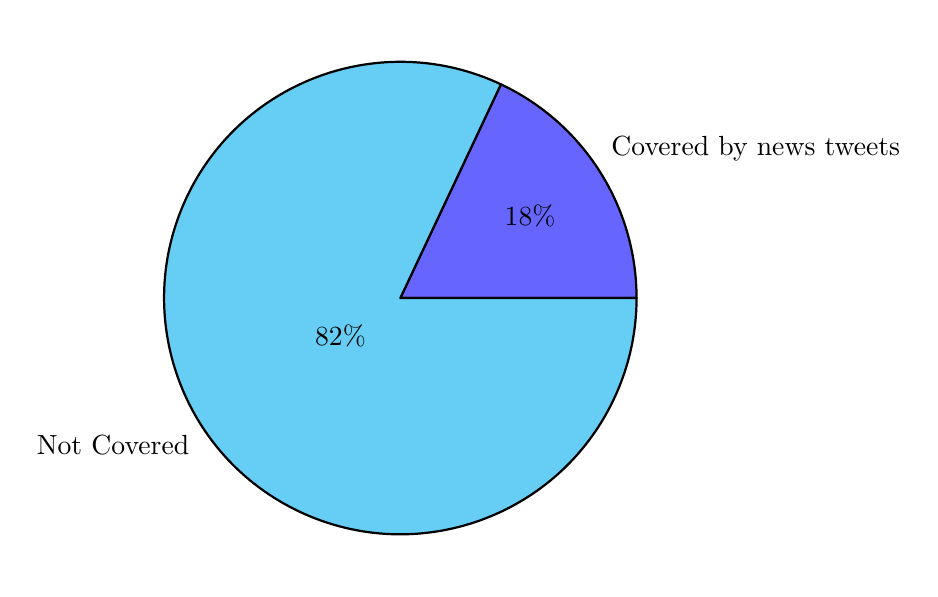
\begin{tikzpicture}
 \pie [rotate = 0]
    {18/ Covered by news tweets,
     82/ Not Covered}
\end{tikzpicture}
\end{figure}

\pagebreak
\section{Data Gathering}

For each of the 470 tweets from USGS, data was compiled for:

\begin{itemize}
    \item first related news tweet (if any)
    \item magnitude of earthquake
    \item location of earthquake
\end{itemize}

This was joined with data on 629 indices from around the world, from four different asset classes. These indicies have been identified by Bloomberg as being the major global, regional and local indices for their respective asset classes. Table~\ref{tab:assetclasses} shows the breakdown of by asset class. 

\begin {table}[H]
\caption{Asset Classes Analysed} \label{tab:assetclasses}
\begin{center}
    \begin{tabu}{| c c c c | } 
        \hline
        \rowfont[c]{\bfseries} Asset Class & Trading & Liquidity & Num Indices  \\
        \hline\hline
        Equities & Trading Hours & Medium & 348 \\
        Rates & Trading Hours & Low & 65 \\ 
        FX & 24/7 & High & 168\\
        Commodities & Global Trading & Low & 48 \\
        \hline
    \end{tabu}
\source{Bloomberg L.P.\cite{bloomberg}}
\end{center}
\end{table}

For these indices, their approximate location was calculated using the same methods as the tweets. The full list of indices used and the country they represent can be found in the appendices. Equities in Appendix~\ref{sec.B}, Rates in Appendix~\ref{sec.C}, FX in Appendix~\ref{sec.D}, and Commodities in Appendix~\ref{sec.E}.

When joined with the 470 USGS tweets, we were able to calculate:

\begin{itemize}
    \item Distance from earthquake to the index/exchange
    \item Price changes from the time of the earthquake to the time of the USGS tweet
    \item Price changes from the time of the USGS tweet to the time of the first related news tweet
    \item Price changes every minute after the USGS tweet
\end{itemize}

\pagebreak
\section{Data Mining}

Before testing the data, it needed to be cleaned. All records where the index didn't move because the trading market wasn't open were removed so as to not distort the distributions.

Using dataframes and stats libraries in python, the data can easily be cut and manipulated, to look for significant relationships:

\begin{enumerate}
    \item Do asset classes move in response to an earthquake?
    \item Do any individual indices move in response to earthquakes?
\end{enumerate}

Because a small earthquake in one country is not likely to affect the stock market in a country on the other side of the world, due to proximity and size, those two factors were used for further filtering when searching for patterns:

\begin{enumerate}
    \item Do markets move when a large earthquake occurs?
    \item Do markets move more when large earthquake occurs versus a small one?
    \item Are markets in close proximity affected?
    \item Are markets in close proximity affected more than further markets? Can this be generalised to a certain distance?
    \item Do markets close to an earthquake move more if a large earthquake occurs?
\end{enumerate}

These same parameters were also used to check for potential pair trades; long one instrument and short an alternative. For example, long a local index, but short an index in an unrelated market to adjust for coincidental market moves.

\pagebreak
\section{Hypothesis Testing}

Financial market prices are often considered random with a mean reversion to zero \cite{burton_random_walk}. This is why, for most scenarios, investors are looking for returns either greater than (long position) or less than zero (short position). Which means the hypothesis to test is:

\setcounter{hyp}{-1}
\begin{hyp} \label{hyp:null}That the average return is equal to zero \end{hyp}
\begin{hyp} \label{hyp:alt}That the average return is not equal to zero \end{hyp}

This is a two tailed t-test, using one sample. The significance level chosen is 95\%, so:
\begin{align*}
    \alpha&= (1 - 95\%)/2  \\
    &= 0.025
\end{align*}

Alternatively, prices are sometimes modelled using stochastic differential equations, using the standard deviation of returns, with a drift based on the risk free rate of the asset\cite{Hull_Options}. The hypothesis test for returns equal to zero is still appropriate, as long as the final check includes adjustments for the risk free rate and standard deviation of returns.

For trades entered at the time of the USGS tweet, to the first news tweet, the single sample t-tests run were:

\begin{itemize}
    \item Asset Class returns on aggregate
    \item Asset Class returns given various Richter scale filters
    \item Asset Class returns filtered by indicies close to the epicentre
    \item Single Index returns on aggregate
    \item Single Index returns given various Richter scale filters
    \item Single Index returns filtered by indicies close to the epicentre
\end{itemize}

With 67\% of the earthquakes in the review window registering less than 6 on the Richter scale, scores above six were grouped for investigation. To complete the search, this threshold was increased in increments of 0.1.

To run the tests filtering by those close to the equator, the checks were done starting with those within 2,000km from the epicenter (about 5\% of the earth's circumference. This was increased in increments of 500km up to 20,000, and the hypothesis tests were run.

Section~\ref{subsec:hyp_test} described some of the assumptions behind the t-test, such as size and distribution. For every test performed, the result was not accepted unless the assumptions held. Expanding on Equation~\ref{eq:minpop}, this function was used:

\begin{lstlisting}[caption={Function to test if assumptions hold}, captionpos=t, label={lst:assumpt}]
def assumptions_hold(sample_s, skew, kurt, count):
    # Z score of significance = 1.96
    # margin of error = 5%
    min_p = (1.96**2 * sample_s * (1-sample_s))/(0.05**2)
    #count must be greater than minimum population, skew and kurt must both be close to zero
    return (count > min_p) and (abs(skew) < 0.5) and (abs(kurt) < 2)
\end{lstlisting}

Some tests compared two sets of returns against each other. This sort of analysis can be useful for investors looking to make a long/short trade. The average return of each is compared in a two-sample t-test. In this case the hypothesis is:

\setcounter{hyp}{-1}
\begin{hyp}[Test hypothesis] \label{hyp:null_2}That the average return of the two returns sets is equal \end{hyp}
\begin{hyp} \label{hyp:alt_2}That the average return of the two returns sets is not equal \end{hyp}

For the distance tests, the data was first separated into those below a threshold, and those within a threshold. Three groups were established, and the boundaries were varied which searching the space for significant trades. The three groups were; very-close, neighbouring, and unrelated. 

The circumference of the earth is 40,075km. This means the furthest great circle distance between two points is around 20,000km. Within the same asset class every index located within a certain close distance, was compared with those located within a range. The loop used to search is shown in Listing~\ref{lst:pair_trades}. It shows how boundaries were established and then searched extensively. A similar loop was run for comparing the very-close group to the unrelated group, where the unrelated group was all indices located further than a certain distance away.

\begin{lstlisting}[caption={Searching for significant pair trades}, captionpos=t, label={lst:pair_trades}]
from scipy import stats.f, stats.ttest_ind
alpha = 0.05/2
#earth's circumference is 40,000 km
for i in range(1000, 4000, step=200):
    for j in range(2000,5000, step=200):
        if j>i:
            for each asset, grp in grouped_returns:
                # find close group / near group
                close_grp = grp[(grp['Distance']<=i)].groupby('Ticker')
                near_grp = grp[(grp['Distance']<=j)&(grp['Distance']>i)].groupby('Ticker')
                #find all cross-wise pairs
                for name_c, close in close_grp:
                    for name_n, near in near_grp:
                        #calculate f-stat, t-stat p value, distribution calcs
                        
                        #if assumptions valid & p-value < alpha record details
                    
\end{lstlisting}

The news tweet is the close signal for the trade, and the USGS tweet is the open signal. As discussed previously, there were many cases where earthquakes were not covered by the media. This would lead to a open trade without a finite close signal. Because of this, an alternate close signal was investigated. Of the earthquakes covered, over 50\% were picked up by news agencies within 40 minutes. So, for each earthquake, prices movements for 40 minutes afterwards were analysed, and searched for significant returns.


%When writing the Methods section  must clearly identify the statistical methods  will use to generate the results needed to meet the research objectives and the research scope.
%²  must also demonstrate that  understand all assumptions associated with the methods  used and justify why those methods are appropriate for r research.
%² For example,  cannot just state \Bootstrapping methods will be used to generate con¯dence intervals for the population correlation coe±cient."  need to show that r study meets the necessary assumptions to use bootstrapping methods to generate con¯dence intervals for the population correlation coe±cient.
%² Remember that `methods' are di®erent than `results'. Therefore,  should not be presenting summaries (such as tables and ¯gures of results) in the Methods chapter. 
%Do cannot assume that r committee members or anyone who will read the dissertation understands the methods  used. Therefore, in the Methods chapter,  should Clearly describe the methods.  should provide enough details so that anyone %reading the dissertation would know how to replicate r research.
%Justify why the statistical methods are appropriate.
%Include simple examples that demonstrate an application of methods.
 % Data Analysis

\chapter{Results}

\section{Network Training}

The first stage of training was search for the better topology regions. It also involved confirming the best activation functions to use.

\subsection{Optimising Topology and Activation Functions}

Table~\ref{tab:leaky_perf} shows the best networks trained using leaky ReLU in the hidden layers. Learning rates of 0.01, 0.05 and 0.1 were all tested, 0.01 was the best.

\begin {table}[H]
\caption{Leaky ReLU Best performance, lr=0.01} \label{tab:leaky_perf}
\begin{center}
    \begin{tabu}{| r r r r r | }
        \hline
        \rowfont[c]{\bfseries} First & Second & Epochs & Alpha & Loss \\
        \hline\hline
            3 & 2 & 100 & 0.1 & 8.40\% \\ \hline
            4 & 2 & 100 & 0.1 & 8.42\% \\ \hline
            4 & 4 & 100 & 0.1 & 8.47\% \\ \hline
            4 & 4 & 100 & 0.2 & 8.71\% \\ \hline
            2 & 2 & 100 & 0.1 & 9.23\% \\ \hline
            3 & 3 & 100 & 0.1 & 9.95\% \\ \hline
    \end{tabu}
\end{center}
\end{table}

\begin{figure}[H]
\caption{Leaky ReLU performance with Learning Rate 0.01}
\label{fig:leaky}
\centering
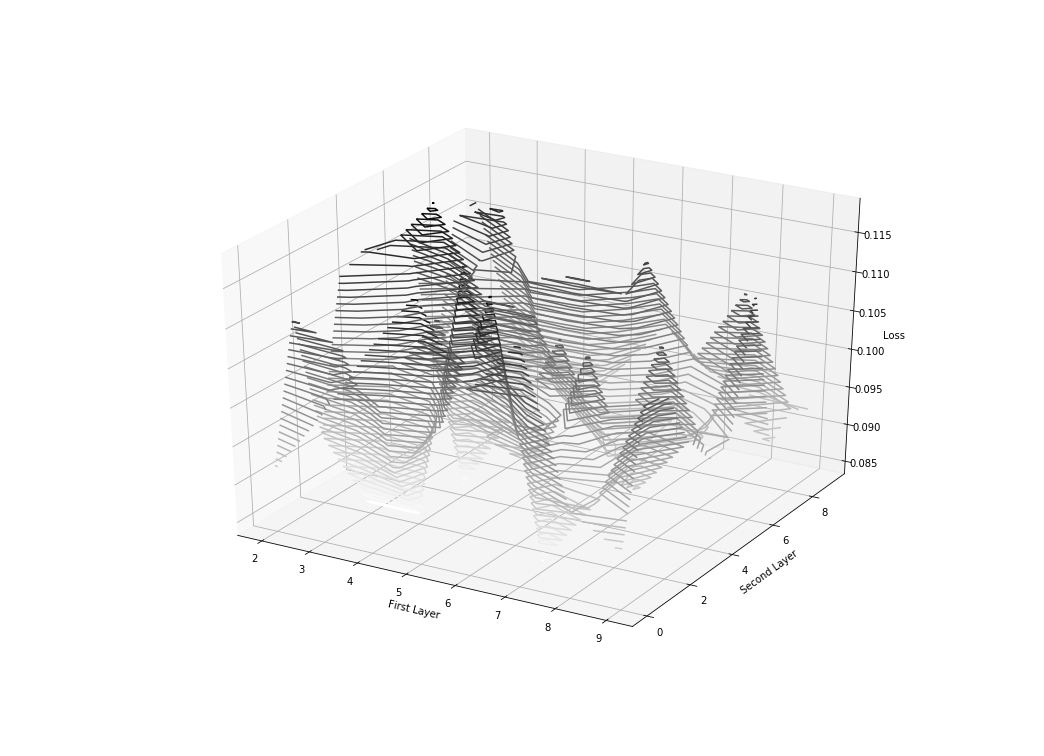
\includegraphics[width=1.0\textwidth]{Figures/leaky.png}
\end{figure}

Table~\ref{tab:tanh_perf} shows the performance when training with the tanh function. Tanh performed very poorly as an activation function on the output layer. Even though tanh is centered around zero, this should not have affected the training as the purpose of the bias unit is to assist in a shift on the y-axis. One possible additional test for this is to re-encode the False signals to $-1$, but given that tanh is a scaled version of sigmoid, sigmoid can be used instead.

\begin {table}[H]
\caption{Tanh Best performance, lr=0.01} \label{tab:tanh_perf}
\begin{center}
    \begin{tabu}{| r r r r r | }
        \hline
        \rowfont[c]{\bfseries} First & Second & Learning Rate & Epochs & Loss \\
        \hline\hline
            2 & 2 & 0.01 & 100 & 106.69\% \\ \hline
            3 & 1 & 0.01 & 100 & 106.69\% \\ \hline
            2 & 1 & 0.01 & 100 & 133.67\% \\ \hline
            2 & 2 & 0.05 & 100 & 149.52\% \\ \hline
            2 & 1 & 0.05 & 100 & 149.52\% \\ \hline
            3 & 1 & 0.05 & 100 & 149.52\% \\ \hline
    \end{tabu}
\end{center}
\end{table}

Using the combination of ReLU as the activation function for hidden layers, and sigmoid as the activation function at the final layer was the best result.

\begin {table}[H]
\caption{Sigmoid Best performance} \label{tab:sigmoid_perf}
\begin{center}
    \begin{tabu}{| r r r r r | }
        \hline
        \rowfont[c]{\bfseries} First & Second & Learning Rate & Epochs & Loss \\
        \hline\hline
            3 & 2 & 0.01 & 56 & 6.03\% \\ \hline
            3 & 1 & 0.01 & 92 & 6.04\% \\ \hline
            5 & 0 & 0.01 & 73 & 6.13\% \\ \hline
            7 & 2 & 0.01 & 50 & 6.13\% \\ \hline
            10 & 2 & 0.01 & 60 & 6.26\% \\ \hline
            4 & 1 & 0.01 & 38 & 6.32\% \\ \hline
            2 & 2 & 0.01 & 73 & 6.32\% \\ \hline
            8 & 0 & 0.05 & 93 & 6.35\% \\ \hline
            6 & 4 & 0.01 & 84 & 6.37\% \\ \hline
            4 & 0 & 0.01 & 100 & 6.38\% \\ \hline
    \end{tabu}
\end{center}
\end{table}

\begin{figure}[H]
\caption{Network Topology affect on Loss Function}
\label{fig:topology_loss}
\centering
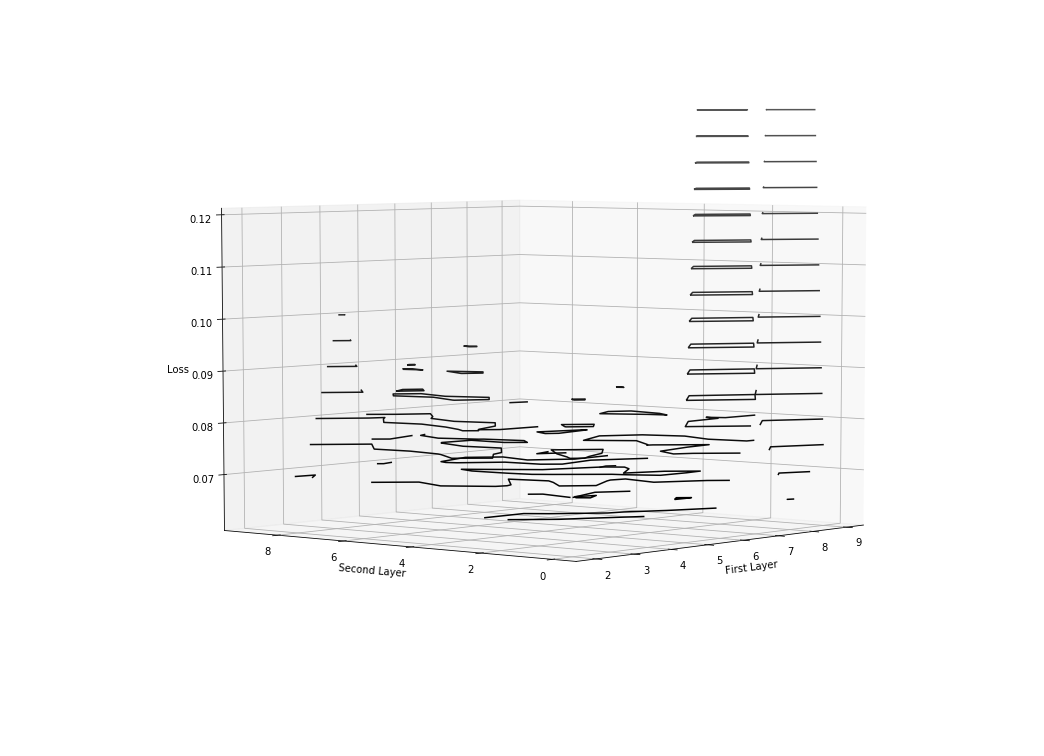
\includegraphics[width=1.0\textwidth]{Figures/sigmoid_chart.png}
\end{figure}

Figure~\ref{fig:nodesVloss}, shows the slight positive correlation ($\rho =0.4$) between the loss function on the test set, and the number of total nodes in a network. This shows the more nodes in a network, the more likely it is to over-fit the data. A simpler, generalised solution is more likely to have predictive power on an unseen data set.

\begin{figure}[H]
    \centering
    \caption{Total Hidden Nodes Vs Loss Function}
    \label{fig:nodesVloss}
        \begin{tikzpicture}
        \begin{axis} [enlargelimits=true, x tick label style={
            /pgf/number format/.cd,
                fixed,
                fixed zerofill,
                precision=0,
                /tikz/.cd
            },
            ymin=0,
            xmin=0,
            xlabel={Total Nodes},
            ylabel={Loss (\%)}
            ]
        \addplot+[
            only marks,
            scatter,
            mark= o,
            mark size=2.9pt]
        table {Data/NodesLR.dat};
        \end{axis}
        \end{tikzpicture}
\end{figure}

\subsection{Hyper-parameters}

The next iteration was to search more possibilities for the learning rate, and also test with a momentum term. Table~\ref{tab:momentum_perf} shows the results using two hidden layers; three nodes in the first hidden layer, and two nodes in the second.

\begin {table}[H]
\caption{Best performance adjusting Momentum} \label{tab:momentum_perf}
\begin{center}
    \begin{tabu}{| r r r r | }
        \hline
        \rowfont[c]{\bfseries} Epochs & Learning Rate & Momentum & Loss \\
        \hline\hline
            35 & 0.010 & 0.6 & 7.99\% \\ \hline
            27 & 0.009 & 0.5 & 8.00\% \\ \hline
            18 & 0.009 & 0.7 & 8.06\% \\ \hline
            25 & 0.011 & 0.7 & 8.06\% \\ \hline
            13 & 0.006 & 0.8 & 8.09\% \\ \hline
    \end{tabu}
\end{center}
\end{table}

\begin{figure}[H]
\caption{Effect of learning rate and momentum on the Loss Function}
\label{fig:leaky}
\centering
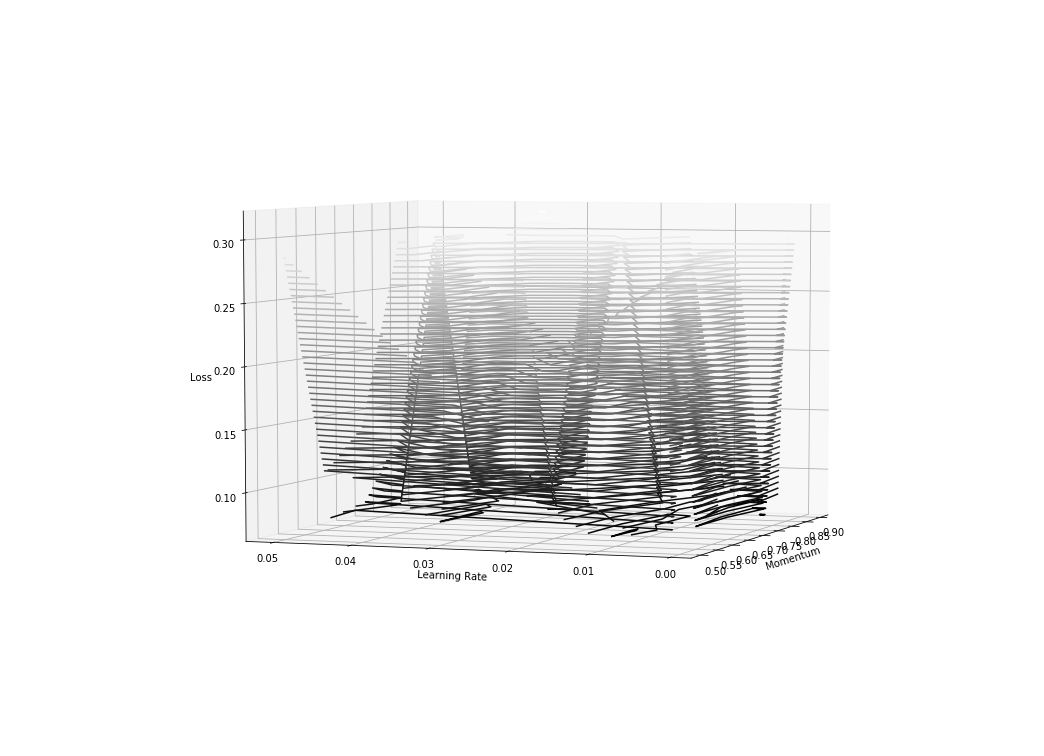
\includegraphics[width=1.0\textwidth]{Figures/momentum_test.png}
\end{figure}

Momentum did not appear to help find a global minimum, but it did help speed the training up, and converge faster.

Focusing on the learning rate, the best rate seemed to be between 0.001 and 0.1 as per Figure~\ref{fig:loss_learn}.

\begin{figure}[H]
\caption{Learning Rate vs Loss}  \label{fig:loss_learn} 
\centering
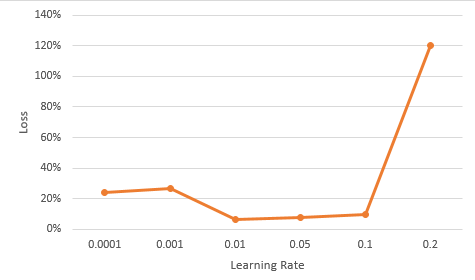
\includegraphics[width=0.8\textwidth]{Figures/LearningRate1.PNG}
\end{figure}

After narrowing the range using the learning rate with no momentum, the results is shown in figure~\ref{fig:narrow_LR}. This shows that the best learning rate for this network is still 0.01.

\begin{figure}[H]
\caption{Narrow Learning Rate Search}  \label{fig:narrow_LR} 
\centering
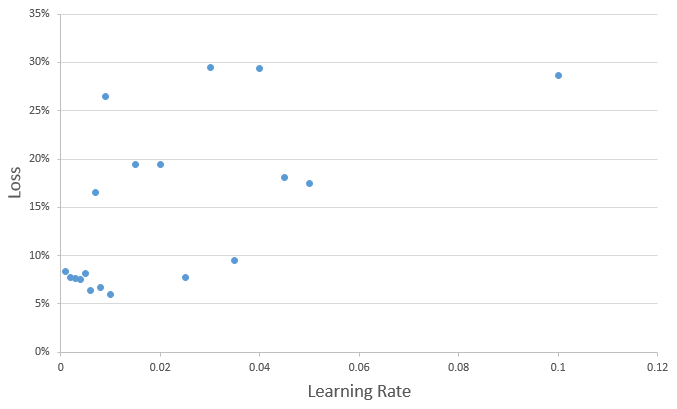
\includegraphics[width=0.8\textwidth]{Figures/LearningRate2.PNG}
\end{figure}

Figure~\ref{fig:learningrate} compares the same model topology, but with a different learning rate. The best performing model tested quickly moved along the cost function and was stopped early. With a much higher learning rate, the second test didn't converge, even after running for 200 epochs.

\begin{figure}[H]
    \centering
    \caption{Evidence of the effect of accurate learning rate}
    \label{fig:learningrate}
        \begin{tikzpicture}
        \begin{axis} [enlargelimits=false,
            y tick label style={
                /pgf/number format/.cd,
                fixed,
                fixed zerofill,
                precision=2,
                /tikz/.cd
            },
            ymin=0,
            xlabel=Epochs,
		    ylabel=Validation Loss,
            ]
        \addplot+[mark= +,
            mark size=2pt
            ]
        table[meta=Oscillates] {Data/LossFunction.dat};
        \addplot+[mark= x,
            mark size=2pt
            ]
        table[meta=Converges] {Data/LossFunction2.dat};
        \legend{$lr=0.2$,$lr=0.01$}
        \end{axis}
        \end{tikzpicture}
\end{figure}

\subsection{Trained Model}

Figure~\ref{fig:modelviz} shows the Keras visualisation of the model with the lowest loss on the test set.

\begin{figure}[H]
\caption{Keras Model vizualisation}  \label{fig:modelviz} 
\centering
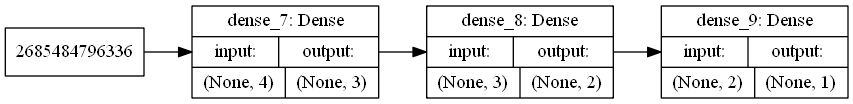
\includegraphics[width=0.8\textwidth]{Figures/model.png}
\source{Keras \cite{chollet2015keras}}
\end{figure}

This same model is graphically displayed in figure \ref{fig:fullmodel}. The weights on each connection of this model are in Table~\ref{tab:weights}.

\begin{sidewaysfigure}
\caption{Final Model Vizualisation}  \label{fig:fullmodel} 
\centering
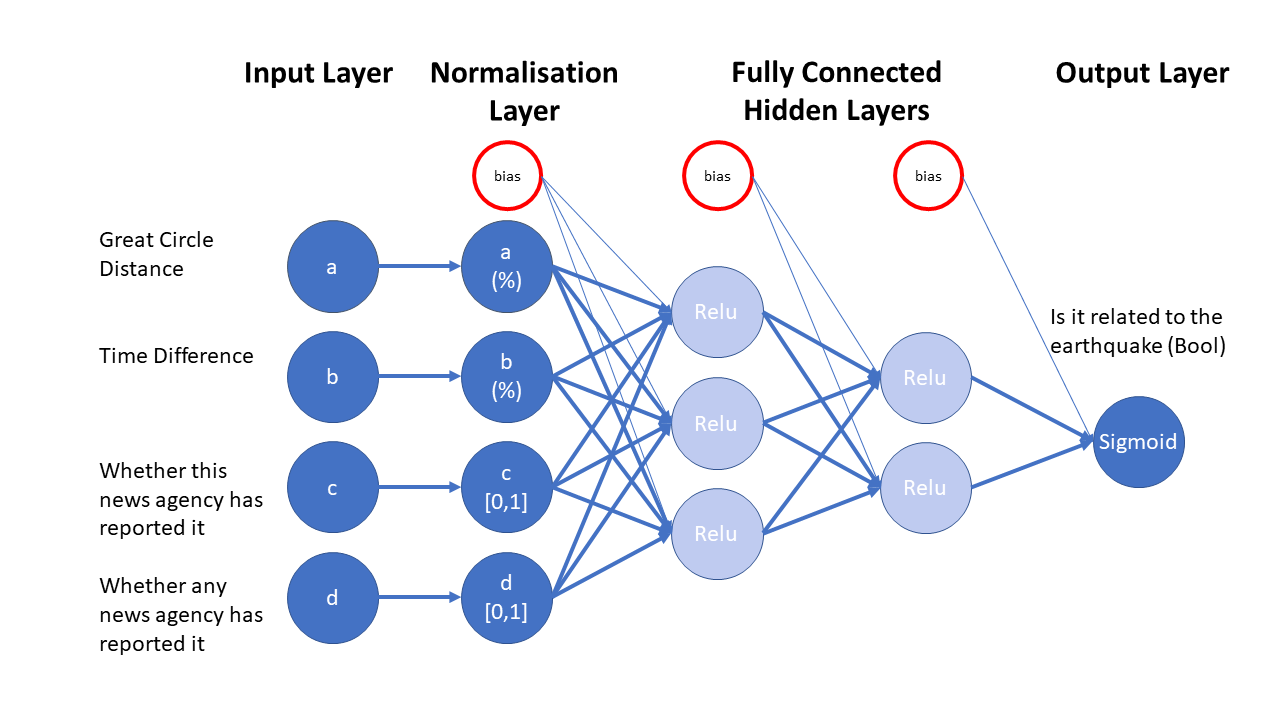
\includegraphics[width=0.9\textwidth]{Figures/FinalNetwork.png}
\end{sidewaysfigure}

\begin {table}[H]
\caption{Best Model Weights} \label{tab:weights}
\begin{center}
\begin{tabu}{l | r r r}
{} & \multicolumn{3}{c}{Nodes} \\
Hidden Layer 1 & 0 & 1 & 2 \\
\hline
0 & -0.64314 & 2.01097 & -0.70205 \\
1 & -0.84878 & 5.35289 & -1.27414 \\
2 & 0.80032 & -0.15045 & -0.23485 \\
3 & 0.02895 & 0.17063 & 0.6392 \\
bias & 0.17831 & 0.06045 & 0.33984 \\
\multicolumn{4}{c}{} \\
{} & \multicolumn{3}{c}{Nodes} \\
Hidden Layer 2 & 0 & 1 & {} \\
\hline
0 & -0.3866 & -1.17079 & {} \\
1 & 2.83778 & 0.99092 & {} \\
2 & -0.90759 & 0.38192 & {} \\
bias & 0.36265 & -0.11841 & {} \\
\multicolumn{4}{c}{} \\
{} & \multicolumn{3}{c}{Nodes} \\
Output & 0 & {} & {} \\
\hline
0 & -2.31861 & {} & {} \\
1 & -1.13171 & {} & {} \\
bias & 2.08073 & {} & {} \\
\end{tabu}
\end{center}
\end{table}

\subsection{Interpreting Predictions}

The objective of training the neural network, was to find a way to systematically predict the sell signal for a trade. Because the system outputs a probability, and the target is a binary, the predictions need to be mapped to a value using thresholding, as discussed in chapter 2.

It is up to the individual practitioner if a decision is required on each tweet. If it is, the standard ROC graph can be used. This ROC graph is shown in figure~\ref{fig:threshold} and shows the relationship between false positives and true positives at different thresholds.

\begin{figure}[H]
    \centering
    \caption{ROC chart for standard threshold tests}
    \label{fig:threshold}
        \begin{tikzpicture}
        \begin{axis} [enlargelimits=false,
            y tick label style={
                /pgf/number format/.cd,
                fixed,
                fixed zerofill,
                precision=2,
                /tikz/.cd
            },
            x tick label style={
                /pgf/number format/.cd,
                fixed,
                fixed zerofill,
                precision=2,
                /tikz/.cd
            },
            ymin=0,
            xmin=0,
            xlabel=fp rate,
		    ylabel=tp rate,
            ]
        \addplot+[mark= +,
            mark size=2pt
            ]
        table[meta=fp_rate] {Data/ROC.dat};
        \addplot+[mark= x,
            mark size=1pt
            ]
        table[meta=tp_rate] {Data/ROC.dat};
        \end{axis}
        \end{tikzpicture}
\end{figure}

In this case, the threshold that produced the largest Area-under-curve was 85\%. This value gave a tp rate of 93.5\% and an fp rate of only 5.3\%, for an AUC of 88.6\%.

Table~\ref{tab:prediction} shows the breakdown of the predictions of the selected model on the testing data set at different threshold levels allowing for an undefined reading. It shows how a wider band not only reduces the errors, but also reduces the accurate predictions.

\begin {table}[H]
\caption{Prediction Precision} \label{tab:prediction}
\begin{center}
    \begin{tabu}{| r r r r r r r | }
        \hline
        \rowfont[c]{\bfseries} Actual & Prediction & 0.5 & $\pm$0.1 & $\pm$0.2 & $\pm$0.3 & $\pm$0.4 \\
        \hline\hline
        FALSE & FALSE & 89.4\% & 88.6\% & 88.3\% & 87.0\% & 86.2\% \\
        TRUE & FALSE & 1.5\% & 0.5\% & 0.3\% & 0.1\% & 0.0\% \\
        FALSE & TRUE & 2.0\% & 0.9\% & 0.4\% & 0.2\% & 0.0\% \\
        TRUE & TRUE & 7.1\% & 6.2\% & 5.9\% & 4.4\% & 0.0\% \\
        \hline
        {} & Total & 100.0\% & 96.3\% & 95.0\% & 91.7\% & 86.2\% \\
        \hline
    \end{tabu}
\end{center}
\end{table}

When plotted, with the adjusted tp, it gives the ROC graph shown in figure~\ref{fig:threshold_adj}.

\begin{figure}[H]
    \centering
    \caption{ROC chart for threshold tests allowing a middle range of un-defined}
    \label{fig:threshold_adj}
        \begin{tikzpicture}
        \begin{axis} [enlargelimits=false,
            y tick label style={
                /pgf/number format/.cd,
                fixed,
                fixed zerofill,
                precision=2,
                /tikz/.cd
            },
            x tick label style={
                /pgf/number format/.cd,
                fixed,
                fixed zerofill,
                precision=3,
                /tikz/.cd
            },
            ymin=0,
            xmin=0,
            xlabel=fp rate,
		    ylabel=tp rate,
            ]
        \addplot+[mark= +,
            mark size=2pt
            ]
        table[meta=fp_rate] {Data/ROC_adj.dat};
        \addplot+[mark= x,
            mark size=1pt
            ]
        table[meta=tp_rate] {Data/ROC_adj.dat};
        \end{axis}
        \end{tikzpicture}
\end{figure}

For this ROC graph, the threshold that produced the largest Area-under-curve was 50$\pm$2\%. This value gave a tp rate of 78.3\% and an fp rate of only 1.3\%, for an AUC of only 77.3\%.

\pagebreak
\section{Data Mining Results}

\subsection{Significant returns against all earthquakes}

Due to the nature of trading hours for many of these instruments, it is very possible that an earthquake happens while markets are closed, and so no one is able to capitalise. As previously discussed FX markets are open 24 hours, 7 days a week, and most commodities are able to be traded in some way during the work week.

Despite this, the below commodity indices have a clear relationship with shock events and prices of base metals tend to drop, straight after an earthquake. Table~\ref{tab:commods_significance_pre} shows that the only indices to move significantly, prior to the USGS tweet are commodities. It is very important to note that these global commodity markets are the first to react to earthquakes. Likely for fundamental reasons such as the potential disruption to supply chains. However, from a trading point of view the return was not worth the risks, as seen by the sharpe ratios less than one.

In this table, and the other tables showing returns, if a return is negative, profits can be made by taking the short position at open and closing the trade with a buy.

\begin {table}[H]
\caption{Significant returns to all earthquakes \textit{before} the USGS tweet} \label{tab:commods_significance_pre}
\begin{center}
    \begin{tabu}{| l l r r r r r | }
        \hline
        \rowfont[c]{\bfseries} Asset & Name & t-stat & p & Rtrn & StDev & Sharpe \\
        \hline \hline
        Commod & SUGAR \#11 (WORLD) & -5.8 & 0.000 & -2.3\% &4.6\% & -0.50 \\
        Commod & LME NICKEL 3MO (\$) & -7.04 & 0.000 & -2.4\% &4.1\% & -0.59 \\
        Commod & Singapore 180 Cst Fuel Month 1 & -5.33 & 0.000 & -1.3\% &3.4\% & -0.39 \\
        Commod & Low Su Gasoil G & -2.81 & 0.006 & -0.4\% &1.5\% & -0.27 \\
        Commod & LME COPPER 3MO (\$) & -2.24 & 0.027 & -0.8\% &4.1\% & -0.20 \\
        Commod & Palladium Spot  \$/Oz & -2.02 & 0.046 & -0.6\% &3.9\% & -0.16 \\
        Commod & GASOLINE RBOB FUTURE & 2.43 & 0.017 & 0.4\% &2.8\% & 0.14 \\
        Commod & ALUMINUM FUTURE & 4.81 & 0.000 & 1.0\% &2.6\% & 0.38 \\
    \hline
    \end{tabu}
    \source{Bloomberg L.P.\cite{bloomberg}}
\end{center}
\end{table}

After the USGS tweet, the base metal prices start to revert after the disruption. Some agricultural commodity markets that didn't move significantly prior to the USGS signal dropped in this second time frame. These trades also had too much risk for the potential return.

\begin {table}[H]
\caption{Significant returns to all earthquakes \textit{after} the USGS tweet.} \label{tab:commods_significance_post}
\begin{center}
    \begin{tabu}{| l l r r r r r | }
        \hline
        \rowfont[c]{\bfseries} Asset & Name & t-stat & p & Rtrn & StDev & Sharpe \\
        \hline \hline
        Commod & WHEAT FUTURE(CBT) & -9.25 & 0.000 & -5.5\% &6.8\% & -0.81 \\
        Commod & CATTLE FEEDER FUTURE & -2.63 & 0.010 & -0.5\% &2.3\% & -0.22 \\
        Commod & COTTON NO.2 FUTURE & -2.03 & 0.045 & -0.7\% &4.2\% & -0.17 \\
        Commod & BRENT CRUDE FUTURE & 1.99 & 0.049 & 0.4\% &2.8\% & 0.14 \\
        Commod & LME COPPER 3MO (\$) & 2.1 & 0.038 & 0.8\% &4.9\% & 0.16 \\
        Commod & Singapore 180 Cst Fuel Month 1 & 5.14 & 0.000 & 1.4\% &3.9\% & 0.36 \\
        Commod & LME NICKEL 3MO (\$) & 6.2 & 0.000 & 2.1\% &4.5\% & 0.46 \\
        Commod & NATURAL GAS FUTURE & 9.71 & 0.000 & 1.4\% &2.7\% & 0.51 \\
        Commod & SUGAR \#11 (WORLD) & 6.01 & 0.000 & 2.5\% &4.8\% & 0.52 \\
    \hline
    \end{tabu}
    \source{Bloomberg L.P.\cite{bloomberg}}
\end{center}
\end{table}

\subsection{Significant Returns against local earthquakes}

Filtering the time series from earthquake to when the USGS announced it by the distance from the epicentre show that equity indices are more susceptible to local movements, than global. 5000km was used as the threshold for nearby indices in the case of the one tailed test. The below indices had more consistent returns as can be seen by the higher sharpe ratios. The Japanese market, through the Nikkei 225 and Nikkei 400, was more susceptible to movements after an earthquake, and with more consistency. Orange juice futures also had more high excess returns for the unit risk.

\begin {table}[H]
\caption{Significant returns to nearby earthquakes} \label{tab:near_eq_significance_pre}
\begin{center}
    \begin{tabu}{| l l r r r r r | }
        \hline
        \rowfont[c]{\bfseries} Asset & Name & t-stat & p & Rtrn & StDev & Sharpe \\
        \hline \hline
        Eq & NIKKEI 225 & 12.21 & 0.000 & 2.5\% &1.6\% & 1.56 \\
        Eq & JPX Nikkei Index 400 & 23.11 & 0.000 & 2.0\% &1.3\% & 1.53 \\
        Commod & FCOJ-A FUTURE & 6.63 & 0.000 & 2.2\% &1.3\% & 1.48 \\
        Eq & NYSE FINANCIAL INDEX & 2.73 & 0.029 & 1.4\% &1.6\% & 0.87 \\
        Eq & TAIWAN TAIEX INDEX & 2.84 & 0.012 & 1.5\% &2.1\% & 0.71 \\
    \hline
    \end{tabu}
    \source{Bloomberg L.P.\cite{bloomberg}}
\end{center}
\end{table}

\subsection{Significant Pair Trades}

Despite this, the experiment was not able to find any significant pair trade ideas by comparing indices located close to the epicenter with those further away.

It is interesting to note that filtering by the magnitude of the earthquake didn't help to produce significant results. Whether grouping by asset class, or looking at individual indices, there was no significant movements when filtered by earthquakes above 6, 6.5 or 7 on the Richter scale.

\subsection{Significant Returns directly after the USGS tweets}

When testing the minute data after the USGS tweet, patterns similar to the first tests emerged. Commodity prices seem to be highly affected by earthquakes, however these ones were large negative movements after the USGS tweet.It usually took over 30 minutes for a significant movement to be found.

\begin {table}[H]
\caption{Asset price changes minute data } \label{tab:minute_data}
\begin{center}
    \hspace*{-2cm}\begin{tabu}{| l l r r r r r r | }
        \hline
        \rowfont[c]{\bfseries} Asset & Name & Minutes & t-stat & p & Rtrn & StDev & Sharpe \\
        \hline \hline
Commod & LME NICKEL 3MO (\$) & 31 & -14.4 & 0.000 & -3.0\% & 2.2\% & -1.37 \\ 
Commod & GASOLINE RBOB FUTURE & 33 & -13.7 & 0.000 & -3.4\% & 2.6\% & -1.29 \\ 
Commod & WHEAT FUTURE(CBT) & 40 & -12.6 & 0.000 & -8.0\% & 6.7\% & -1.2 \\ 
Commod & CORN FUTURE & 40 & -12.2 & 0.000 & -6.0\% & 5.2\% & -1.15 \\ 
Commod & NY Harb ULSD Future & 40 & -11.3 & 0.000 & -1.4\% & 1.3\% & -1.07 \\ 
Commod & ZINC FUT (SHFE) & 35 & -11.0 & 0.000 & -5.6\% & 5.3\% & -1.06 \\ 
Commod & WTI CRUDE FUTURE & 38 & -10.1 & 0.000 & -1.1\% & 1.2\% & -0.96 \\ 
Commod & ALUMINUM FUTURE & 40 & -8.3 & 0.000 & -1.5\% & 1.8\% & -0.82 \\ 
Commod & FCOJ-A FUTURE & 40 & -6.4 & 0.000 & -1.1\% & 1.8\% & -0.63 \\ 
Commod & BRENT CRUDE FUTURE & 38 & -6.3 & 0.000 & -0.7\% & 1.1\% & -0.61 \\ 
Commod & NATURAL GAS FUTURE & 40 & -5.1 & 0.000 & -1.0\% & 2.0\% & -0.49 \\ 
Commod & SUGAR \#11 (WORLD) & 40 & -4.3 & 0.000 & -1.4\% & 3.2\% & -0.42 \\ 
Commod & Palladium Spot  \$/Oz & 33 & -3.2 & 0.002 & -1.1\% & 3.7\% & -0.3 \\ 
Commod & COFFEE 'C' FUTURE & 38 & -2.9 & 0.004 & -1.4\% & 4.9\% & -0.29 \\ 
Commod & Deformed Bar Future & 40 & -2.3 & 0.022 & -1.3\% & 5.7\% & -0.22 \\ 
Commod & SILVER FUTURE & 38 & -2.2 & 0.028 & -0.7\% & 3.3\% & -0.22 \\ 
Commod & Silver Spot  \$/Oz & 38 & -2.2 & 0.033 & -0.6\% & 3.0\% & -0.21 \\ 
Commod & PALLADIUM FUTURE & 39 & 2.3 & 0.022 & 0.7\% & 3.3\% & 0.22 \\ 
    \hline
    \end{tabu}
    \source{Bloomberg L.P.\cite{bloomberg}}
    \hspace*{-2cm}
\end{center}
\end{table}

%chart of returns per minute?
These results are promising, and show that there can be excess returns gained from trading signals generated through earthquake analysis.




%In the Results chapter  describe and summarize the results  found.
%² Remember to include comments that remind r committee that r results satisfy r research objectives and research scope.
%² Whenever possible, use graphical methods to summarize results. For example, it is difficult to see patterns with tables. Results in tables should be supplemented with graphs, plots, ¯gures, ...
%² When presenting speci¯c results,  should mention the research objective that is related to those results.
%² By the end of the Results chapters,  want r committee to know that  have satis¯ed all research objectives and research scope.
 % Results and Discussion

\chapter{Discussion and Conclusion}

The results of this project has shown two things:

\begin{enumerate}
    \item It is possible to identify tweets related to a certain event, such as an earthquake
    \item There are significant market moves on the back of these events
\end{enumerate}

The topology of the final model in terms of number of nodes in the hidden layers was shown to be the best combination for most of the hyper-parameter combinations tried. Even with different activation functions the two layer model [3, 2] was still the best combination. Also, even with different nodes and set-ups the best learning rate was around 0.01. This can give us confidence that the best model was found.

A review of the rules-of-thumb discussed in section~\ref{subsubsec:topology} compared with the optimal model generated shows that it is consistent. The number of hidden layer neurons is at least 2/3 of the size of the input layer, but less than twice that number. Also, the size of each hidden layer is between the layer's input size and the layer's output size. Whilst this doesn't guarantee the model is optimal, it is strong corroborative evidence.

The model weights output show that the inputs for distance and time are more important in deducing whether a tweet is related or not to the earthquake. This was expected.

The two different thresholding approaches yielded very different results, but because the first method had a higher AUC, the standard threshold cutoff of 85\% is recommended.

The existence of significant moves in financial markets after an earthquake, even for trades where the sharpe ratio was less than one, suggest these signals are being generated correctly. Further study on instruments outside the major indices for each asset class can be conducted, specifically derivative instruments and structured products based on these underlyings that could potentially boost returns per unit risk.

\pagebreak
Despite the success of meeting the objectives stated in chapter 1, there are many areas that can be improved on.

One of the constraints was time spent in manually classifying the news tweets. With further resources, the training set could be expanded and potentially take tweets in other languages.

One of the drawbacks in the analysis was that so many of the earthquakes reported, were not actually covered by the fifteen news agencies selected. Running in real-time, with the same trained model, the Twitter handles covered could include all news agencies, and potentially more sources as well. The use of Polyglot libraries for NER will allow the system to use 40 major languages. This would all increase the likelihood of getting a close signal to the trade. Additionally, the Polyglot library could potentially be used to extract earthquake related entities, instead of the list of earthquake related words. This would reduce the number of steps involved, especially for multiple languages, and possibly speed up the analysis.

It is possible that more data will be available within the tweets as Twitter is working on increasing the character limit from 140 to 280. The 140 character limit was an arbitrary threshold because twitter started as an SMS-based service. More characters means that the news agencies could write more details in their announcements and provide more information to the NLP system. Given how news agencies currently uses twitter just for quick headlines for their \#breaking news, this is not expected to have a large effect on the predictive power of the network, but is worth monitoring.

This success is confirmation of the success other teams have had in using twitter feeds for sentiment analysis. As NLP libraries and NER analysis improves, these short form tweets will become more significant for generating trade signals. This will possibly lead to the risk that as more investors use this data as a signal, the markets will move even faster to an efficient price, and opportunities for profits are reduced.

From all the significant trades generated, the ones investors are mostly likely to act on are when there is an earthquake near Japan. Two equity indices increased consistently after the USGS system reported an earthquake. The high incidence of earthquakes in the region means that there was more samples to chose from which increased the chance of having a significant number of data points. Whilst the equity markets are only open a portion of each day, if an earthquake occurs outside market hours, it is less likely to cause as much damage as people will be inside at home, not on the streets.

The other index to move significantly after earthquakes in the region was frozen concentrated orange juice. Because of the potential for spoilage if there are delays in the supply chain for this product, it is logical for investors to price in any potential collapse in logistics.

For the trades generated and analysed by the system, there are some very promising results. The movements of commodities initially, and then after the USGS tweet are logical from a fundamentals point of view. As discussed in Chapter 2, this asset class trades in most markets and time-zones, so it has more availability for trades at times when other markets might be closed. However, this result requires more research as it could have another signal, other than the USGS tweet and is possibly a case of spurious correlation.

Fundamentally, it is likely that commodity markets are affected by earthquakes close to their local region. Particularly bulk commodities like agricultural and base metals, there is a high cost of storage and transportation. Earthquakes can disrupt the supply chain, increasing costs by increasing the chance of spoilage, or the logistics expenses.

The results of filtering by equity indices close to the source of the earthquake was expected. Equities are typically affected by local market movements as well as sentiment which as been confirmed by this analysis.

The lack of effect from earthquakes registering high on the Richter scale is something that requires further study. This could be because the precise location is more important than how severe the earthquake's impact is.

For the pair trades based on distance, it's possible that there wasn't a single significant trade found because of the time-zones many of the instruments are dependant on. For example, an earthquake in India will have short term affects locally, but the US market is closed at that time, so there will be less effect there from the earthquake.

When the minute data right after the USGS tweet was examined, there were a number of significant trades in the commodities universe. This suggested that some commodities have a reasonable lag in adjusting to new information, and investors can use this to make profitable trades. However, this needs to be read in conjunction with the movements from the time the earthquake hit to the time of the USGS tweet. The data showed that it's likely there will be a period of over-reaction and correction, that traders can profit from.

There were no trades generated for the rates class. This is not unusual given that this class is much less volatile than the others, and is less likely to make a significant move on the back of an earthquake. The only exception might be an extremely large one located near a major population area. The lack of trades generated for the FX asset class was not expected. Given the liquidity of this asset class, it is most likely that new information is priced in faster. This could mean that the FX market is much more efficient than other asset classes, pricing in new information faster.

The most important caveat is that entering and exiting positions in short team trades like this are highly dependant on market liquidity. As previously mentioned this paper isn't looking into the market micro structure for this analysis. Given the analysis is on major indices, liquidity will usually not be a problem.

As mentioned in Chapter 4, this paper looked at traditional hypothesis testing methods for establishing significant returns. If objective benchmarks can be established, and implementation bias reduced, tests suggested by Keogh and Kasetty\cite{data_mining_Keogh} are potentially available. There is also the possibility of employing unsupervised machine learning techniques such as k-means clustering to attempt to establish a relationship between the data sets when the issues with machine learning in financial markets highlighted by Zhang and Zhou\cite{golden_nuggets} are overcome.

The profitable trades suggested for tickers in the commodities and equities asset classes after an earthquake suggest that there is alpha available to technologically sophisticated investors. Further work can be done to test the market liquidity after an earthquake, to confirm that slippage and other trading costs do not negate the potential profits.


%The Discussion is much more than a restatement of the research results. Your goal is to help your committee understand what all of the results mean (\see the big picture").
%You have the opportunity to review your work as a whole.
%² You need to relate the contents of the Results chapter to the Literature Review chapter. That is, you want to compare and contrast your results to the contents of the important references that you cited.
%² You want to show to your committee that you can interpret your research results (and not just summarize the results). That is, you want to convince your committee that your results are truly analyzed (and not only described).
%² You should also indicate any limitations of your research (such as reviewing the research scope) that researchers need to address in the future.
%² In the Discussion, it must be clear if a statement you make is a direct result of your research results (within the scope) or if you are generalizing beyond the research scope.

%In writing the conclusions you should restate your principal findings, the importance of your findings in the academic field and explain how your research question/s have been answered by the methods you employed and the evidence you have found. To a certain extent this will replicate the introduction; in that it is a summary. Neither introduction nor the conclusion can outline anything in detail: both act as guides to the content within the rest of the dissertation.

 % Conclusion


%% ----------------------------------------------------------------
% Now begin the Appendices, including them as separate files

\addtocontents{toc}{\vspace{2em}} % Add a gap in the Contents, for aesthetics

\appendix % Cue to tell LaTeX that the following 'chapters' are Appendices

%\chapter{Sample USGS Tweets} \label{sec.A} 
\begin {table}[H]
\begin{center}
    \hspace*{-2cm}\begin{tabu}{|c c c c c|} 
        \hline
        \rowfont[c]{\bfseries} Coordinates & Date & Magnitude & Region & Time-stamp \\ \hline
        \hline\hline
        (-5.746, 150.767) & 17-12-30 08:15 & 5.7 & New Britain, Papua New Guinea & 17-12-29 23:55 \\ \hline
        (-20.0, -115.0) & 17-12-30 05:41 & 5.7 & southern East Pacific Rise & 17-12-29 21:20 \\ \hline
        (4.306, 126.803) & 17-12-29 01:36 & 5.7 & Kepulauan Talaud, Indonesia &  17-12-28 17:20 \\ \hline
        (-23.650, -70.397) & 17-12-28 12:11 & 5.5 & the coast of Antofagasta, Chile & 17-12-28 03:54 \\ \hline
        (13.524, 144.823) & 17-12-28 08:16 & 5.5 & Guam region & 17-12-27 23:58 \\ \hline
        (33.171, 139.771) & 17-12-21 11:12 & 5.7 & Izu Islands, Japan region & 17-12-21 03:00 \\ \hline
        (33.743, 133.637) & 17-12-20 21:57 & 5.5 & southeast of Shikoku, Japan & 17-12-20 13:40 \\ \hline
        (9.555, 138.139) & 17-12-18 07:55 & 5.5 & Federated States of Micronesia & 17-12-17 23:41 \\ \hline
        (0.0, -20.0) & 17-12-16 22:57 & 5.5 & central Mid-Atlantic Ridge & 17-12-16 14:38 \\ \hline
        (-7.614, 110.712) & 17-12-16 01:06 & 6.5 & Java, Indonesia & 17-12-15 16:47 \\ \hline
        (-21.041, 167.271) & 17-12-15 04:55 & 5.5 & southeast of the Loyalty Islands & 17-12-14 20:36 \\ \hline
        (-20.202, -69.287) & 17-12-12 03:18 & 5.5 & coast of Tarapaca, Chile & 17-12-11 19:00 \\ \hline
        (-15.376, 166.959) & 17-12-12 01:45 & 5.7 & Vanuatu & 17-12-11 17:29 \\ \hline
        (-21.178, -175.198) & 17-12-11 19:11 & 5.6 & Tonga & 17-12-11 10:50 \\ \hline
        (9.555, 138.139) & 17-12-09 23:32 & 6.1 & Federated States of Micronesia & 17-12-09 15:14 \\ \hline
        (-21.178, -175.198) & 17-12-09 07:59 & 5.7 & Tonga & 17-12-08 23:42 \\ \hline
        (9.555, 138.139) & 17-12-08 18:08 & 6.4 & Federated States of Micronesia & 17-12-08 09:51 \\ \hline
        (9.555, 138.139) & 17-12-08 13:57 & 5.5 & Federated States of Micronesia & 17-12-08 05:37 \\ \hline
        (-29.266, -177.916) & 17-12-08 10:28 & 6.2 & Kermadec Islands, New Zealand & 17-12-08 02:09 \\ \hline
        (9.555, 138.139) & 17-12-08 08:39 & 6.5 & Federated States of Micronesia & 17-12-08 00:22 \\ \hline
        (-1.847, 120.527) & 17-12-07 00:24 & 5.5 & Sulawesi, Indonesia & 17-12-06 16:06 \\ \hline
        (-5.012, 141.347) & 17-12-01 11:09 & 6 & eastern New Guinea region & 17-12-01 02:50 \\ \hline
        (0.0, -20.0) & 17-11-30 14:50 & 6.7 & central Mid-Atlantic Ridge  & 17-11-30 06:32 \\ \hline
        (-5.012, 141.347) & 17-11-30 14:08 & 5.5 & New Guinea, Papua New Guinea & 17-11-30 05:50 \\ \hline
        (-5.703, 126.609) & 17-11-30 08:11 & 5.5 & Banda Sea & 17-11-29 23:53 \\ \hline
        (33.543, -117.782) & 17-11-29 14:45 & 5.7 & near the coast of central Peru & 17-11-29 06:29 \\ \hline
        \hline

    \end{tabu}
    \source{Twitter, processed by GetOldTweets \cite{getoldtweets}}
    \hspace*{-2cm}
\end{center}
\end{table}


	% USGS Tweets

\chapter{List of Equity Indices} \label{sec.B}

Major World Equity Indices from Bloomberg's WEI$<GO>$ function\cite{bloomberg}.

\begin {table}[H]
\begin{center}
\small
\hspace*{-3cm}
\begin{tabu}{| l l l |} 
\hline
Ticker & Name & Country\\
\hline
INDU Index & DOW JONES INDUS. AVG & UNITED STATES \\ 
TRAN Index & DOW JONES TRANS. AVG & UNITED STATES \\ 
UTIL Index & DOW JONES UTILITY AVG & UNITED STATES \\ 
COMP Index & DOW JONES COMP. AVG & UNITED STATES \\ 
DWCF Index & DJTSM US & UNITED STATES \\ 
OEX Index & S\&P 100 INDEX & UNITED STATES \\ 
SPX Index & S\&P 500 INDEX & UNITED STATES \\ 
MID Index & S\&P 400 MIDCAP INDEX & UNITED STATES \\ 
SML Index & S\&P 600 SMALLCAP INDEX & UNITED STATES \\ 
SPR Index & S\&P 1500 Composite Index & UNITED STATES \\ 
NYA Index & NYSE COMPOSITE INDEX & UNITED STATES \\ 
NYID Index & NYSE U.S. 100 INDEX & UNITED STATES \\ 
NYIID Index & NYSE INTERNATIONAL 100 & UNITED STATES \\ 
NYYID Index & NYSE TMT INDEX & UNITED STATES \\ 
NYLID Index & NYSE WORLD LEADERS INDX & UNITED STATES \\ 
VALUA Index & Value Line Arithmetic & UNITED STATES \\ 
CCMP Index & NASDAQ COMPOSITE INDEX & UNITED STATES \\ 
CFIN Index & NASDAQ OTHER FINANCIAL & UNITED STATES \\ 
NYP Index & NYSE HEALTHCARE INDEX & UNITED STATES \\ 
NYK Index & NYSE FINANCIAL INDEX & UNITED STATES \\ 
CIND Index & NASDAQ INDUSTRIAL INDEX & UNITED STATES \\ 
CTRN Index & NASDAQ TRANSPORTATION IX & UNITED STATES \\ 
CUTL Index & NASDAQ TELECOMM INDEX & UNITED STATES \\ 
CINS Index & NASDAQ INSURANCE INDEX & UNITED STATES \\ 

\hline
\end{tabu}
\hspace*{-3cm}
\small
\end{center}
\end{table}

\begin {table}[H]
\begin{center}
\small
\hspace*{-3cm}
\begin{tabu}{| l l l |} 
\hline
Ticker & Name & Country\\
\hline
CBNK Index & NASDAQ BANK INDEX & UNITED STATES \\ 
NDX Index & NASDAQ 100 STOCK INDX & UNITED STATES \\ 
NDF Index & NASDAQ FINANCIAL INDEX & UNITED STATES \\ 
IXK Index & NASDAQ COMPUTER INDEX & UNITED STATES \\ 
NBI Index & NASDAQ BIOTECH INDEX & UNITED STATES \\ 
QMI Index & NASDAQ 100 PRE-MKT IDX & UNITED STATES \\ 
QIV Index & NASDAQ 100 AFTER HOUR IX & UNITED STATES \\ 
XMI Index & NYSE Arca Major Market & UNITED STATES \\ 
XAX Index & NYSE AMER COM & UNITED STATES \\ 
XII Index & NYSE Arca Institutional & UNITED STATES \\ 
XCI Index & NYSE Arca Computer Tech & UNITED STATES \\ 
XOI Index & NYSE Arca Oil & UNITED STATES \\ 
BBREIT Index & BBG US REITS & UNITED STATES \\ 
OSX Index & OIL SERVICE SECTOR INDEX & UNITED STATES \\ 
RIY Index & RUSSELL 1000 INDEX & UNITED STATES \\ 
RTY Index & RUSSELL 2000 INDEX & UNITED STATES \\ 
RAY Index & RUSSELL 3000 INDEX & UNITED STATES \\ 
XAU Index & PHILA GOLD \& SILVER INDX & UNITED STATES \\ 
SOX Index & PHILA SEMICONDUCTOR INDX & UNITED STATES \\ 
BKX Index & KBW BANK INDEX & UNITED STATES \\ 
UTY Index & PHILA UTILITY INDEX & UNITED STATES \\ 
SPTSX Index & S\&P/TSX COMPOSITE INDEX & CANADA \\ 
TXEQ Index & S\&P/TSX EQUITY INDEX & CANADA \\ 
SPTSX60 Index & S\&P/TSX 60 INDEX & CANADA \\ 
SPTSXVEN Index & S\&P/TSX VENTURE COMP IDX & CANADA \\ 
MEXBOL Index & S\&P/BMV IPC & MEXICO \\ 
INMEX Index & S\&P/BMV INMEX & MEXICO \\ 
IMC30 Index & S\&P/BMV MidCap Select 30 & MEXICO \\ 
IRT Index & S\&P/BMV IRT & MEXICO \\ 
FTBIVA Index & FTSE BIVA PR & MEXICO \\ 
BVPSBVPS Index & Bolsa de Panama General & PANAMA \\ 
MERVAL Index & ARGENTINA MERVAL INDEX & ARGENTINA \\ 
BURCAP Index & ARGENTINA BURCAP INDEX & ARGENTINA \\ 
MAR Index & M.AR MERVAL ARGENTINA IX & ARGENTINA \\ 
IBG Index & INDICE BOLSA GENERAL & ARGENTINA \\ 
IBOV Index & BRAZIL IBOVESPA INDEX & BRAZIL \\ 
IBX Index & BRAZIL IBrX INDEX & BRAZIL \\ 
IBOVIEE Index & BRAZIL ELECTRIC.ENRGY IX & BRAZIL \\ 
IGCX Index & BRAZIL CORP GOV INDEX & BRAZIL \\ 
IVBX2 Index & BRAZIL VAL/BOV 2 TIER IX & BRAZIL \\ 
IBX50 Index & BRAZIL IBrX-50 INDEX & BRAZIL \\ 
IPSA Index & S\&P/CLX IPSA (CLP) TR & CHILE \\ 
IGPA Index & S\&P/CLX IGPA (CLP) TR & CHILE \\ 
INTER10 Index & S\&P/CLX INTER-10 CLP TR & CHILE \\ 
CHILE65 Index & CHILE 65 INDEX & CHILE \\ 

\hline
\end{tabu}
\hspace*{-3cm}
\small
\end{center}
\end{table}

\begin {table}[H]
\begin{center}
\small
\hspace*{-3cm}
\begin{tabu}{| l l l |} 
\hline
Ticker & Name & Country\\
\hline
CHLRGCAP Index & CHILE LARGE CAP INDEX & CHILE \\ 
CHSMLCAP Index & CHILE SMALL CAP INDEX & CHILE \\ 
IBVC Index & VENEZUELA STOCK MKT INDX & VENEZUELA \\ 
SPBLPGPT Index & S\&P/BVLPeruGeneralTRPEN & PERU \\ 
SPBL25PT Index & S\&P/BVLLIMA25TRPEN & PERU \\ 
COLCAP Index & COLOMBIA COLCAP INDEX & COLOMBIA \\ 
COLSC Index & Colombia COLSC index & COLOMBIA \\ 
COLIR Index & Colombia COLIR Index & COLOMBIA \\ 
COLEQTY Index & Colombia COLEQTY  Index & COLOMBIA \\ 
BSX Index & BERMUDA STOCK EXCHANGE & BERMUDA \\ 
JMSMX Index & JSE MARKET INDEX & JAMAICA \\ 
BE500 Index & BLOOMBERG EUROPEAN 500 & EUROZONE \\ 
SX5E Index & Euro Stoxx 50 Pr & EUROZONE \\ 
SX5P Index & STXE 50 € Pr & EUROZONE \\ 
SXXE Index & ESTX € Pr & EUROZONE \\ 
SXXP Index & STXE 600 € Pr & EUROZONE \\ 
EUE15P Index & STX EUEnlrg 15 € Pr & EUROZONE \\ 
EUETMP Index & STX EUEnlrg TM € Pr & EUROZONE \\ 
E100 Index & FTSE EUROTOP 100 INDEX & EUROZONE \\ 
E300 Index & FTSEUROFIRST 300 INDEX & EUROZONE \\ 
MSER Index & MSCI EURO & EUROZONE \\ 
MSPE Index & MSCI PAN-EURO & EUROZONE \\ 
SPEURO Index & S\&P EUROPE 350 INDEX & EUROZONE \\ 
SPEU Index & S\&P EURO INDEX & EUROZONE \\ 
BWORLDEU Index & BBG EMEA WORLD INDEX & UNITED STATES \\ 
N100 Index & EURONEXT TOP 100 INDEX & EUROZONE \\ 
N150 Index & EURONEXT TOP 150 INDEX & EUROZONE \\ 
FTEF80 Index & FTSEurofirst 80  Index & EUROZONE \\ 
FTEFC1 Index & FTSEurofirst 100 Index & EUROZONE \\ 
NTX Index & NEW EUROPE BLUE CHIP IX & EUROZONE \\ 
UKX Index & FTSE 100 INDEX & BRITAIN \\ 
MCX Index & FTSE 250 INDEX & BRITAIN \\ 
NMX Index & FTSE 350 INDEX & BRITAIN \\ 
SMX Index & FTSE SMALLCAP INDEX & BRITAIN \\ 
ASX Index & FTSE ALL-SHARE INDEX & BRITAIN \\ 
T1X Index & FTSE techMARK Focus Ix & BRITAIN \\ 
AXX Index & FTSE AIM ALL SHARE INDEX & BRITAIN \\ 
DAX Index & DAX INDEX & GERMANY \\ 
CDAX Index & GERM CDAX  PERFORMANCE & GERMANY \\ 
HDAX Index & HDAX INDEX & GERMANY \\ 
MDAX Index & MDAX PERF INDEX & GERMANY \\ 
TDXP Index & TECDAX PERFORMANCE INDEX & GERMANY \\ 
PXAP Index & PRIME ALL SHARE PRF IDX & GERMANY \\ 
MIDP Index & MIDCAP MRKT PERF INDEX & GERMANY \\ 

\hline
\end{tabu}
\hspace*{-3cm}
\small
\end{center}
\end{table}


\begin {table}[H]
\begin{center}
\small
\hspace*{-3cm}
\begin{tabu}{| l l l |} 
\hline
Ticker & Name & Country\\
\hline
NMDP Index & TECHLGY ALL SHARE PRF IX & GERMANY \\ 
CLXP Index & CLASSIC ALL SHARE PRF IX & GERMANY \\ 
CAC Index & CAC 40 INDEX & FRANCE \\ 
SBF250 Index & CAC All-Tradable & FRANCE \\ 
CN20 Index & CAC NEXT 20 INDEX & FRANCE \\ 
CM100 Index & CAC Mid 60 Index & FRANCE \\ 
MS190 Index & CAC Mid \& Small Index & FRANCE \\ 
CS90 Index & CAC Small Index & FRANCE \\ 
PAX Index & CAC ALLSHARES INDEX & FRANCE \\ 
SBF120 Index & SBF 120 INDEX & FRANCE \\ 
IBEX Index & IBEX 35 INDEX & SPAIN \\ 
MADX Index & SPAIN MA  MADRID INDEX & SPAIN \\ 
ES30 Index & DJ SPAIN TITANS 30 € & SPAIN \\ 
SMI Index & SWISS MARKET INDEX & SWITZERLAND \\ 
SPI Index & SPI SWISS PERFORMANCE IX & SWITZERLAND \\ 
CH30 Index & DJ SWISS TITANS 30 S? & SWITZERLAND \\ 
SPIEXX Index & SPI EXTRA PRICE RETURN & SWITZERLAND \\ 
SMIM Index & SMIM PRICE INDEX & SWITZERLAND \\ 
SLI Index & SLI SWISS LEADER INDEX & SWITZERLAND \\ 
FTSEMIB Index & FTSE MIB INDEX & ITALY \\ 
ITLMS Index & FTSE Italia All-Share & ITALY \\ 
ITMC Index & FTSE Italia Mid Cap Ind & ITALY \\ 
ITSTAR Index & FTSE Italia STAR Index & ITALY \\ 
IT30 Index & DJ ITALY TITANS 30 € & ITALY \\ 
BVLX Index & PSI All-Share Index GR & PORTUGAL \\ 
PSI20 Index & PSI 20 INDEX & PORTUGAL \\ 
ISEQ Index & IRISH OVERALL INDEX & IRELAND \\ 
ICEXI Index & OMX Iceland All-Share PR & ICELAND \\ 
AEX Index & AEX-Index & NETHERLANDS \\ 
AMX Index & AMSTERDAM MIDKAP INDEX & NETHERLANDS \\ 
BEL20 Index & BEL 20 INDEX & BELGIUM \\ 
BELSTK Index & BEL All-Share NR & BELGIUM \\ 
LUXXX Index & LUXEMBOURG LuxX INDEX & LUXEMBOURG \\ 
LUXXR Index & LUXEMBOURG LuxX RETURN & LUXEMBOURG \\ 
KFX Index & OMX COPENHAGEN 20 INDEX & DENMARK \\ 
KAX Index & OMX COPENHAGEN INDEX & DENMARK \\ 
OMXC25 Index & OMX Copenhagen 25 Index & DENMARK \\ 
HEX Index & OMX HELSINKI INDEX & FINLAND \\ 
HEX25 Index & OMX HELSINKI 25 INDEX & FINLAND \\ 
HEXP Index & OMXHCap & FINLAND \\ 
OBX Index & OBX STOCK INDEX & NORWAY \\ 
OBXP Index & OBX PRICE INDEX & NORWAY \\ 
OSEAX Index & OSE ALL SHARE INDEX & NORWAY \\ 


\hline
\end{tabu}
\hspace*{-3cm}
\small
\end{center}
\end{table}


\begin {table}[H]
\begin{center}
\small
\hspace*{-3cm}
\begin{tabu}{| l l l |} 
\hline
Ticker & Name & Country\\
\hline
OSEBX Index & OSE BENCHMARK INDEX & NORWAY \\ 
OSEFX Index & OSE MUTUAL FUND INDEX & NORWAY \\ 
OSESX Index & OSE SMALL CAP INDEX & NORWAY \\ 
OMXO20GI Index & OMX Oslo 20 GI Index & NORWAY \\ 
OMXO20 Index & OMX Oslo 20 Index & NORWAY \\ 
OMX Index & OMX STOCKHOLM 30 INDEX & SWEDEN \\ 
SBX Index & OMX STOCKHOLM BENCHMARK & SWEDEN \\ 
SAX Index & OMX Stockholm All-Share & SWEDEN \\ 
SE30 Index & DJ SWEDEN TITANS 30 SEK & SWEDEN \\ 
ATX Index & AUSTRIAN TRADED ATX INDX & AUSTRIA \\ 
WBI Index & AUSTRIAN VIENNA STOCK EX & AUSTRIA \\ 
ATXPRIME Index & AUSTRIAN ATX PRIME INDEX & AUSTRIA \\ 
ASE Index & Athex Composite Share Pr & GREECE \\ 
FTASE Index & FTSE/ASE Large Cap & GREECE \\ 
FTSEM Index & FTSE/ASE MIDCAP INDEX & GREECE \\ 
WIG Index & WSE WIG INDEX & POLAND \\ 
WIG20 Index & WIG 20 & POLAND \\ 
SWIG80 Index & WSE sWIG80 INDEX & POLAND \\ 
MIDWIG Index & WSE mWIG40 INDEX & POLAND \\ 
PX Index & PRAGUE STOCK EXCH INDEX & CZECH \\ 
IMOEX Index & MOEX Russia Index & RUSSIA \\ 
MICEX10 Index & MICEX 10 INDEX & RUSSIA \\ 
RTSI\$ Index & RUSSIAN RTS INDEX \$ & RUSSIA \\ 
RTSSTD Index & RTS Standard Index & RUSSIA \\ 
CRTX Index & RUSSIAN TRADED INDEX & RUSSIA \\ 
BUX Index & BUDAPEST STOCK EXCH INDX & HUNGARY \\ 
CHTX Index & HUNGARIAN TRADED INDEX & HUNGARY \\ 
BET Index & BUCHAREST BET INDEX & ROMANIA \\ 
PFTS Index & PFTS Index & UKRAINE \\ 
UX Index & Ukrainian Equities Index & UKRAINE \\ 
KZKAK Index & Kazakhstan KASE Stock Ex & KAZAKHSTAN \\ 
SKSM Index & SLOVAK SHARE INDEX & SLOVAKIA \\ 
CRO Index & CROATIA ZAGREB CROBEX & CROATIA \\ 
SBITOP Index & Slovenian Blue Chip Idx & SLOVENIA \\ 
BIRS Index & Bosnia BIRS Index & BOSNIA-HERZE. \\ 
SASX10 Index & SASE Free Market 10 Idx & BOSNIA-HERZE. \\ 
BELEXLIN Index & BELEXline Index & Serbia \\ 
BELEX15 Index & BELEX15 INDEX & Serbia \\ 
TALSE Index & OMX TALLINN OMXT & ESTONIA \\ 
MBI Index & MBI 10 Index & MACEDONIA \\ 
RIGSE Index & OMX RIGA OMXR & LATVIA \\ 
VILSE Index & OMX VILNIUS OMXV & LITHUANIA \\ 
SOFIX Index & SOFIX INDEX & BULGARIA \\ 

\hline
\end{tabu}
\hspace*{-3cm}
\small
\end{center}
\end{table}


\begin {table}[H]
\begin{center}
\small
\hspace*{-3cm}
\begin{tabu}{| l l l |} 
\hline
Ticker & Name & Country\\
\hline
XU100 Index & BIST 100 INDEX & TURKEY \\ 
XU030 Index & BIST 30 Index & TURKEY \\ 
TR20I Index & DJ TURKEY TITANS 20 & TURKEY \\ 
CYSMMAPA Index & GENERAL MARKET INDEX CSE & CYPRUS \\ 
MALTEX Index & MALTA STOCK EXCHANGE IND & MALTA \\ 
TOP40 Index & FTSE/JSE AFRICA TOP40 IX & SOUTH AFRICA \\ 
JALSH Index & FTSE/JSE AFRICA ALL SHR & SOUTH AFRICA \\ 
INDI25 Index & FTSE/JSE AFRICA IND25 IX & SOUTH AFRICA \\ 
HERMES Index & EGYPT HERMES INDEX & EGYPT \\ 
EGX30 Index & EGX 30 INDEX & EGYPT \\ 
MOSENEW Index & MASI Free Float Index & MOROCCO \\ 
MOSEMDX Index & MADEX Free Float Index & MOROCCO \\ 
TUSISE Index & Tunis SE TUNINDEX & TUNISIA \\ 
FTN098 Index & NAMIBIA OVERALL INDEX & NAMIBIA \\ 
BGSMDC Index & Botswana Gaborone Dom & BOTSWANA \\ 
NGSEINDX Index & NIGERIA STCK EXC ALL SHR & NIGERIA \\ 
DARSDSEI Index & Tanzania All Share Index & TANZANIA \\ 
KNSMIDX Index & Nairobi SE 20 Share & KENYA \\ 
NSEASI Index & Nairobi All Share & KENYA \\ 
GGSECI Index & GSE Composite Index & GHANA \\ 
KWSEPM Index & KWSE Premier Mkt & KUWAIT \\ 
KWSEMM Index & KWSE Main Mkt & KUWAIT \\ 
TA-35 Index & TA-35 Index & ISRAEL \\ 
TA-125 Index & TA-125 Index & ISRAEL \\ 
PASISI Index & PSE Al Quds & PALESTINE \\ 
BLOM Index & BLOM STOCK INDEX & LEBANON \\ 
BHSEASI Index & BB ALL SHARE INDEX & BAHRAIN \\ 
SASEIDX Index & TADAWUL ALL SHARE INDEX & SAUDI ARABIA \\ 
JOSMGNFF Index & AMMAN SE GENERAL INDEX & JORDAN \\ 
MSM30 Index & MSM30 Index & OMAN \\ 
DSM Index & QE Index & QATAR \\ 
QEAS Index & QE All Share Index & QATAR \\ 
QETR Index & QE Total Return Index & QATAR \\ 
DFMGI Index & DFM GENERAL INDEX & UAE \\ 
ADSMI Index & ADX GENERAL INDEX & UAE \\ 
DUAE Index & FTSE NASDAQ DUB UAE 20 & UAE \\ 
SEMDEX Index & MAURITIUS STOCK EXCHANGE & MAURITIUS \\ 
TPX Index & TOPIX INDEX (TOKYO) & JAPAN \\ 
NKY Index & NIKKEI 225 & JAPAN \\ 
JPNK400 Index & JPX Nikkei Index 400 & JAPAN \\ 
HSI Index & HANG SENG INDEX & HONG KONG \\ 
SHSZ300 Index & CSI 300 INDEX & CHINA \\ 
SHCOMP Index & SHANGHAI SE COMPOSITE & CHINA \\ 


\hline
\end{tabu}
\hspace*{-3cm}
\small
\end{center}
\end{table}


\begin {table}[H]
\begin{center}
\small
\hspace*{-3cm}
\begin{tabu}{| l l l |} 
\hline
Ticker & Name & Country\\
\hline
SZCOMP Index & SHENZHEN SE COMPOSITE IX & CHINA \\ 
HSCEI Index & HANG SENG CHINA ENT INDX & HONG KONG \\ 
TWSE Index & TAIWAN TAIEX INDEX & TAIWAN \\ 
KOSPI Index & KOSPI INDEX & SOUTH KOREA \\ 
KOSDAQ Index & KOSDAQ INDEX & SOUTH KOREA \\ 
AS51 Index & S\&P/ASX 200 INDEX & AUSTRALIA \\ 
NIFTY Index & Nifty 50 & INDIA \\ 
SENSEX Index & S\&P BSE SENSEX INDEX & INDIA \\ 
SX40 Index & SX40 & INDIA \\ 
STI Index & Straits Times Index STI & SINGAPORE \\ 
FBMKLCI Index & FTSE Bursa Malaysia KLCI & MALAYSIA \\ 
SET Index & STOCK EXCH OF THAI INDEX & THAILAND \\ 
JCI Index & JAKARTA COMPOSITE INDEX & INDONESIA \\ 
NZSE50FG Index & S\&P/NZX 50 Index Gross & NEW ZEALAND \\ 
PCOMP Index & PSEi - PHILIPPINE SE IDX & PHILIPPINES \\ 
KSE100 Index & KARACHI 100 INDEX & PAKISTAN \\ 
VNINDEX Index & HO CHI MINH STOCK INDEX & VIETNAM \\ 
CSEALL Index & SRI LANKA COLOMBO ALL SH & SRI LANKA \\ 
LSXC Index & Laos Composite Index & LAOS \\ 
MSETOP Index & MSE Top 20 Index & MONGOLIA \\ 
SAXCME Index & S\&P ASIA 50 INDEX CME & HONG KONG \\ 
MXAPEXA Index & MSCI ASIA APEX 50 & MULT \\ 
TPX Index & TOPIX INDEX (TOKYO) & JAPAN \\ 
TPXC30 Index & TOPIX CORE 30 IDX (TSE) & JAPAN \\ 
TPXL70 Index & TOPIX LARGE 70 IDX (TSE) & JAPAN \\ 
TPX500 Index & TOPIX 500 INDEX (TSE) & JAPAN \\ 
TPXSM Index & TOPIX SMALL INDEX (TSE) & JAPAN \\ 
TPXM400 Index & TOPIX MID 400 INDX (TSE) & JAPAN \\ 
TPX100 Index & TOPIX 100 INDEX (TSE) & JAPAN \\ 
TSE2 Index & TSE2 TOPIX 2ND SECT INDX & JAPAN \\ 
NKY Index & NIKKEI 225 & JAPAN \\ 
NEY Index & NIKKEI 300 INDEX & JAPAN \\ 
NKY500 Index & NIKKEI 500 & JAPAN \\ 
JSDA Index & JASDAQ: STOCK INDEX & JAPAN \\ 
NKYJQ Index & NIKKEI JASDAQ & JAPAN \\ 
TSEREIT Index & TSE REIT INDEX & JAPAN \\ 
TSEMOTHR Index & TSE MOTHERS INDEX & JAPAN \\ 
JPNK400 Index & JPX Nikkei Index 400 & JAPAN \\ 
HSI Index & HANG SENG INDEX & HONG KONG \\ 
HSCI Index & HANG SENG COMPOSITE INDX & HONG KONG \\ 
HKSPLC25 Index & S\&P/HKEx LargeCap Index & HONG KONG \\ 
HKSPGEM Index & S\&P/HKEx GEM Index & HONG KONG \\ 
HSCEI Index & HANG SENG CHINA ENT INDX & HONG KONG \\ 
HSCCI Index & HANG SENG CHINA AFF.CRP & HONG KONG \\ 

\hline
\end{tabu}
\hspace*{-3cm}
\small
\end{center}
\end{table}


\begin {table}[H]
\begin{center}
\small
\hspace*{-3cm}
\begin{tabu}{| l l l |} 
\hline
Ticker & Name & Country\\
\hline
HSFML25 Index & HS China (HK-listed) 25 & HONG KONG \\ 
H-FIN Index & HANG SENG H-FINANCIALS & HONG KONG \\ 
HSML100 Index & HS China (HK-listed) 100 & HONG KONG \\ 
HSHK35 Index & HANG SENG HK 35 INDEX & HONG KONG \\ 
SHSZ300 Index & CSI 300 INDEX & CHINA \\ 
SHASHR Index & SHANGHAI SE A SHARE INDX & CHINA \\ 
SHBSHR Index & SHANGHAI SE B SHARE INDX & CHINA \\ 
SZASHR Index & SHENZHEN SE A SHARE INDX & CHINA \\ 
SZBSHR Index & SHENZHEN SE B SHARE INDX & CHINA \\ 
SHCOMP Index & SHANGHAI SE COMPOSITE & CHINA \\ 
SZCOMP Index & SHENZHEN SE COMPOSITE IX & CHINA \\ 
SSE180 Index & SHANGHAI SE 180 A SHR IX & CHINA \\ 
SSE50 Index & SSE 50 Index & CHINA \\ 
SHNCOMP Index & SHANGHAI G-SHARES & CHINA \\ 
SICOM Index & SZSE COMPONENT INDEX & CHINA \\ 
SZ399006 Index & ChiNext Price Index & CHINA \\ 
SHCSI100 Index & CSI 100 Index - Shanghai & CHINA \\ 
SZSMEC Index & CHINA SHENZ SM EN CO IDX & CHINA \\ 
SZ399550 Index & CCTV 50 INDEX & CHINA \\ 
SZ399330 Index & SZSE 100 PRICE INDEX SZ & CHINA \\ 
SZ399005 Index & CHINA SHENZ MIDCP EN IDX & CHINA \\ 
SH000905 Index & CSI Smallcap 500 Index & CHINA \\ 
TWSE Index & TAIWAN TAIEX INDEX & TAIWAN \\ 
TWOTCI Index & TAIWAN TPEx EXCHANGE & TAIWAN \\ 
TW50 Index & FTSE TWSE Taiwan 50 Indx & TAIWAN \\ 
KRX100 Index & KRX 100 INDEX & SOUTH KOREA \\ 
KOSPI Index & KOSPI INDEX & SOUTH KOREA \\ 
KOSPI2 Index & KOSPI 200 INDEX & SOUTH KOREA \\ 
KOSPI100 Index & KOREA KOSPI 100 INDEX & SOUTH KOREA \\ 
KOSPI50 Index & KOREA KOSPI 50 INDEX & SOUTH KOREA \\ 
KOSDAQ Index & KOSDAQ INDEX & SOUTH KOREA \\ 
AS51 Index & S\&P/ASX 200 INDEX & AUSTRALIA \\ 
AS52 Index & S\&P/ASX 300 INDEX & AUSTRALIA \\ 
AS30 Index & ALL ORDINARIES INDX & AUSTRALIA \\ 
NZSE50FG Index & S\&P/NZX 50 Index Gross & NEW ZEALAND \\ 
NZSE10 Index & S\&P/NZX 10 Index & NEW ZEALAND \\ 
NZSE Index & S\&P NZX All Index & NEW ZEALAND \\ 
KSE100 Index & KARACHI 100 INDEX & PAKISTAN \\ 
KSE30 Index & KARACHI 30 INDEX & PAKISTAN \\ 
KSE Index & KARACHI ALL SHARE INDEX & PAKISTAN \\ 
CSEALL Index & SRI LANKA COLOMBO ALL SH & SRI LANKA \\ 
SET Index & STOCK EXCH OF THAI INDEX & THAILAND \\ 
SET50 Index & THAI SET 50 INDEX & THAILAND \\ 

\hline
\end{tabu}
\hspace*{-3cm}
\small
\end{center}
\end{table}



\begin {table}[H]
\begin{center}
\small
\hspace*{-3cm}
\begin{tabu}{| l l l |} 
\hline
Ticker & Name & Country\\
\hline
JCI Index & JAKARTA COMPOSITE INDEX & INDONESIA \\ 
LQ45 Index & JAKARTA LQ-45 INDEX & INDONESIA \\ 
SENSEX Index & S\&P BSE SENSEX INDEX & INDIA \\ 
NIFTY Index & Nifty 50 & INDIA \\ 
BSE500 Index & S\&P BSE 500 IDX & INDIA \\ 
BSE200 Index & S\&P BSE 200 IDX & INDIA \\ 
BSE100 Index & S\&P BSE 100 IDX & INDIA \\ 
SX40 Index & SX40 & INDIA \\ 
STI Index & Straits Times Index STI & SINGAPORE \\ 
FSTAS Index & FTSE ST ALL SHARE INDEX & SINGAPORE \\ 
FBMKLCI Index & FTSE Bursa Malaysia KLCI & MALAYSIA \\ 
FBMEMAS Index & FTSE BURSA MALAYSIA EMAS & MALAYSIA \\ 
PCOMP Index & PSEi - PHILIPPINE SE IDX & PHILIPPINES \\ 
VNINDEX Index & HO CHI MINH STOCK INDEX & VIETNAM \\ 
VHINDEX Index & HNX INDEX & VIETNAM \\ 
DSEX Index & DSE Broad Index & BANGLADESH \\ 
DS30 Index & DSE 30 Index & BANGLADESH \\ 
MSETOP Index & MSE Top 20 Index & MONGOLIA \\ 
LSXC Index & Laos Composite Index & LAOS \\ 
\hline
\end{tabu}
\hspace*{-3cm}
\small
\end{center}
\end{table}
 % Equity Indices

\chapter{List of Rates Indices} \label{sec.C} 
Major World Bond Markets from Bloomberg's WB$<GO>$ function\cite{bloomberg}.

\begin {table}[H]
\begin{center}
\small
\begin{tabu}{| l l l |} 
\hline
Ticker & Name & Country \\
\hline
AO548092 Corp & CANADIAN GOVERNMENT & CANADA \\
9128284V Govt & US TREASURY N/B & UNITED STATES \\
AR008512 Corp & REPUBLIC OF CHILE & CHILE \\
AM217073 Corp & REPUBLIC OF COLOMBIA & COLOMBIA \\
AQ599663 Corp & UNITED MEXICAN STATES & MEXICO \\
QZ744509 Corp & BONOS DE TESORERIA & PERU \\
AP416684 Corp & FED REPUBLIC OF BRAZIL & BRAZIL \\
EJ509646 Corp & TITULOS DE TESORERIA B & COLOMBIA \\
EG111637 Corp & MEX BONOS DESARR FIX RT & MEXICO \\
AQ617800 Corp & REPUBLIC OF ARGENTINA & ARGENTINA \\
AQ608474 Corp & NOTA DO TESOURO NACIONAL & BRAZIL \\
EH334522 Corp & REPUBLIC OF VENEZUELA & VENEZUELA \\
AS442589 Corp & LITHUANIA GOVERNMNT BOND & LITHUANIA \\
AR263158 Corp & NIGERIA GOVERNMENT BOND & NIGERIA \\
EE190475 Corp & SWITZERLAND & SWITZERLAND \\
AM127829 Corp & KINGDOM OF DENMARK & DENMARK \\
AT428688 Corp & BUNDESREPUB. DEUTSCHLAND & GERMANY \\
AR698279 Corp & NETHERLANDS GOVERNMENT & NETHERLANDS \\
AM216366 Corp & SWEDISH GOVERNMENT & SWEDEN \\
AQ850212 Corp & REPUBLIC OF AUSTRIA & AUSTRIA \\
AM241648 Corp & BULGARIA GOVERNMENT BOND & BULGARIA \\
AU256850 Corp & FINNISH GOVERNMENT & FINLAND \\
AS907838 Corp & FRANCE (GOVT OF) & FRANCE \\
AR150340 Corp & EFSF & LUXEMBOURG \\
\hline
\end{tabu}
\small
\end{center}
\end{table}

\begin {table}[H]
\begin{center}
\small
\begin{tabu}{| l l l |} 
\hline
Ticker & Name & Country \\
\hline
AQ788320 Corp & BELGIUM KINGDOM & BELGIUM \\
AS959205 Corp & SLOVAKIA GOVERNMENT BOND & SLOVAKIA \\
AS769661 Corp & REPUBLIC OF LATVIA & LATVIA \\
AQ595858 Corp & IRISH TSY 2028 & IRELAND \\
AQ603805 Corp & REPUBLIKA SLOVENIJA & SLOVENIA \\
AT282059 Corp & BONOS Y OBLIG DEL ESTADO & SPAIN \\
AR641250 Corp & UK TSY 1 5/8\% 2028 & BRITAIN \\
AQ703194 Corp & OBRIGACOES DO TESOURO & PORTUGAL \\
AS256449 Corp & NORWEGIAN GOVERNMENT & NORWAY \\
AL069977 Corp & ISRAEL FIXED BOND & ISRAEL \\
AM393077 Corp & REPUBLIC OF CROATIA BOND & CROATIA \\
EJ561598 Corp & CZECH REPUBLIC & CZECH \\
AU556558 Corp & REPUBLIC OF CYPRUS & CYPRUS \\
AT758770 Corp & BUONI POLIENNALI DEL TES & ITALY \\
EJ678153 Corp & POLAND GOVERNMENT BOND & POLAND \\
JV526727 Corp & HUNGARY GOVERNMENT BOND & HUNGARY \\
AQ182926 Corp & HELLENIC REPUBLIC & GREECE \\
AP285915 Corp & SAUDI INTERNATIONAL BOND & SAUDI ARABIA \\
AR790243 Corp & RUSSIAN FEDERATION & RUSSIA \\
AU352489 Corp & ROMANIA GOVERNMENT BOND & ROMANIA \\
AM216492 Corp & RIKISBREF & ICELAND \\
AQ692016 Corp & REPUBLIC OF TURKEY & TURKEY \\
EJ525789 Corp & RUSSIA GOVT BOND - OFZ & RUSSIA \\
CP507394 Corp & REPUBLIC OF SOUTH AFRICA & SOUTH AFRICA \\
QJ494644 Corp & LEBANESE REPUBLIC & LEBANON \\
AR547286 Corp & TURKEY GOVERNMENT BOND & TURKEY \\
AU632628 Corp & TAIWAN GOVT RECONSTRUCT & TAIWAN \\
AT427280 Corp & JAPAN (10 YEAR ISSUE) & JAPAN \\
EJ790610 Corp & HONG KONG GOVERNMENT & HONG KONG \\
AR990434 Corp & KOREA TREASURY BOND & SOUTH KOREA \\
AS303943 Corp & SINGAPORE GOVERNMENT & SINGAPORE \\
AR670289 Corp & NEW ZEALAND GOVERNMENT & NEW ZEALAND \\
LW020767 Corp & AUSTRALIAN GOVERNMENT & AUSTRALIA \\
AT454543 Corp & THAILAND GOVERNMENT BOND & THAILAND \\
AT965438 Corp & CHINA GOVERNMENT BOND & CHINA \\
EJ715276 Corp & MALAYSIA GOVERNMENT & MALAYSIA \\
AQ286257 Corp & REPUBLIC OF INDONESIA & INDONESIA \\
AR756595 Corp & PHILIPPINE GOVERNMENT & PHILIPPINES \\
EJ314632 Corp & INDONESIA GOVERNMENT & INDONESIA \\
AQ584277 Corp & INDIA GOVERNMENT BOND & INDIA \\
AL935775 Corp & PAKISTAN INVESTMENT BOND & PAKISTAN \\
\hline
\end{tabu}
\small
\end{center}
\end{table} % Rates Indices

\chapter{List of FX Indices}\label{sec.D} 
Major World Currency Rates from Bloomberg's WCR$<GO>$ function\cite{bloomberg}.

\begin {table}[H]
\begin{center}
\small
\begin{tabu}{| l l || l l |} 
\hline
Ticker & Country & Ticker & Country \\
\hline
USDAFN Curncy & AFGHANISTAN & USDBND Curncy & BRUNEI \\ 
USDALL Curncy & ALBANIA & USDBGN Curncy & BULGARIA \\ 
USDDZD Curncy & ALGERIA & USDBIF Curncy & BURUNDI \\ 
USDADP Curncy & ANDORRA & USDKHR Curncy & CAMBODIA \\ 
USDAOA Curncy & ANGOLA & USDCAD Curncy & CANADA \\ 
USDARS Curncy & ARGENTINA & USDCVE Curncy & CAPE VERDE \\ 
USDAMD Curncy & ARMENIA & USDKYD Curncy & CAYMAN ISLANDS \\ 
USDAWG Curncy & ARUBA & USDXAF Curncy & CENTRAL AFRICA \\ 
USDAUD Curncy & AUSTRALIA & USDCLP Curncy & CHILE \\ 
USDATS Curncy & AUSTRIA & USDCNY Curncy & CHINA \\ 
USDAZN Curncy & AZERBAIJAN & USDCNH Curncy & CHINA \\ 
USDBSD Curncy & BAHAMAS & USDCOP Curncy & COLOMBIA \\ 
USDBHD Curncy & BAHRAIN & USDKMF CMPT Curncy & COMOROS \\ 
USDBDT Curncy & BANGLADESH & USDCRC Curncy & COSTA RICA \\ 
USDBBD Curncy & BARBADOS & USDHRK Curncy & CROATIA \\ 
USDBYR Curncy & BELARUS & USDCUP Curncy & CUBA \\ 
USDBEF Curncy & BELGIUM & USDCZK Curncy & CZECH \\ 
USDBZD Curncy & BELIZE & USDCDF Curncy & DEM.REP. CONGO \\ 
USDBMD Curncy & BERMUDA & USDDKK Curncy & DENMARK \\ 
USDBTN Curncy & BHUTAN & USDDJF Curncy & DJIBOUTI \\ 
USDBOB Curncy & BOLIVIA & USDDOP Curncy & DOMINICAN REPB. \\ 
USDBAM Curncy & BOSNIA-HERZE. & USDXCD Curncy & EAST CARIBBEAN \\ 
USDBWP Curncy & BOTSWANA & USDECS Curncy & ECUADOR \\ 
USDBRL Curncy & BRAZIL & USDEGP Curncy & EGYPT \\ 
USDGBP Curncy & BRITAIN & USDSVC Curncy & EL SALVADOR \\ 

\hline
\end{tabu}
\small
\end{center}
\end{table}

\begin {table}[H]
\begin{center}
\small
\begin{tabu}{| l l || l l |} 
\hline
Ticker & Country & Ticker & Country \\
\hline
USDERN Curncy & ERITREA & USDJOD Curncy & JORDAN \\ 
USDEEK Curncy & ESTONIA & USDKZT Curncy & KAZAKHSTAN \\ 
USDETB Curncy & ETHIOPIA & USDKES Curncy & KENYA \\ 
USDEUR Curncy & EUROZONE & USDKWD Curncy & KUWAIT \\ 
USDFJD Curncy & FIJI & USDKGS Curncy & KYRGYZSTAN \\ 
USDFIM Curncy & FINLAND & USDLAK Curncy & LAOS \\ 
USDFRF Curncy & FRANCE & USDLVL Curncy & LATVIA \\ 
USDXPF Curncy & FRENCH PACIFIC & USDLBP Curncy & LEBANON \\ 
USDGMD CMPT Curncy & GAMBIA & USDLSL Curncy & LESOTHO \\ 
USDGEL Curncy & GEORGIA & USDLRD Curncy & LIBERIA \\ 
USDDEM Curncy & GERMANY & USDLYD Curncy & LIBYA \\ 
USDGHS Curncy & GHANA & USDLTL Curncy & LITHUANIA \\ 
USDGRD Curncy & GREECE & USDLUF Curncy & LUXEMBOURG \\ 
USDGTQ Curncy & GUATEMALA & USDMOP Curncy & MACAU \\ 
USDGNF Curncy & GUINEA & USDMKD Curncy & MACEDONIA \\ 
USDGYD CMPT Curncy & GUYANA & USDMGA Curncy & MADAGASCAR \\ 
USDHTG Curncy & HAITI & USDMWK Curncy & MALAWI \\ 
USDHNL Curncy & HONDURAS & USDMYR Curncy & MALAYSIA \\ 
USDHKD Curncy & HONG KONG & USDMVR Curncy & MALDIVES \\ 
USDHUF Curncy & HUNGARY & USDMRU Curncy & Mauritania \\ 
USDISK Curncy & ICELAND & USDMUR Curncy & MAURITIUS \\ 
USDINR Curncy & INDIA & USDMXN Curncy & MEXICO \\ 
USDIDR Curncy & INDONESIA & USDMDL Curncy & MOLDOVA \\ 
USDIRR Curncy & IRAN & USDMNT Curncy & MONGOLIA \\ 
USDIQD Curncy & IRAQ & USDMAD Curncy & MOROCCO \\ 
USDIEP Curncy & IRELAND & USDMZN Curncy & MOZAMBIQUE \\ 
USDILS Curncy & ISRAEL & USDMMK Curncy & MYANMAR \\ 
USDITL Curncy & ITALY & USDNAD Curncy & NAMIBIA \\ 
USDJMD Curncy & JAMAICA & USDNPR Curncy & NEPAL \\ 
USDJPY Curncy & JAPAN & USDNLG Curncy & NETHERLANDS \\ 
\hline

\end{tabu}
\small
\end{center}
\end{table}

\begin {table}[H]
\begin{center}
\small
\begin{tabu}{| l l || l l |} 
\hline
Ticker & Country & Ticker & Country \\
\hline
USDNZD Curncy & NEW ZEALAND & USDKRW Curncy & SOUTH KOREA \\ 
USDNIO Curncy & NICARAGUA & USDESP Curncy & SPAIN \\ 
USDNGN Curncy & NIGERIA & USDLKR Curncy & SRI LANKA \\ 
USDKPW Curncy & NORTH KOREA & USDSDG Curncy & SUDAN \\ 
USDNOK Curncy & NORWAY & USDSRD Curncy & SURINAME \\ 
USDOMR Curncy & OMAN & USDSZL Curncy & SWAZILAND \\ 
USDPKR Curncy & PAKISTAN & USDSEK Curncy & SWEDEN \\ 
USDPAB Curncy & PANAMA & USDCHF Curncy & SWITZERLAND \\ 
USDPGK Curncy & PAPUA N.GUINEA & USDSYP Curncy & SYRIA \\ 
USDPYG Curncy & PARAGUAY & USDTWD Curncy & TAIWAN \\ 
USDPEN Curncy & PERU & USDTJS Curncy & TAJIKISTAN \\ 
USDPHP Curncy & PHILIPPINES & USDTZS Curncy & TANZANIA \\ 
USDPLN Curncy & POLAND & USDTHB Curncy & THAILAND \\ 
USDPTE Curncy & PORTUGAL & USDTOP Curncy & TONGA \\ 
USDQAR Curncy & QATAR & USDTTD Curncy & TRINIDAD AND TO \\ 
USDRON Curncy & ROMANIA & USDTND Curncy & TUNISIA \\ 
USDRUB Curncy & RUSSIA & USDTRY Curncy & TURKEY \\ 
USDRWF Curncy & RWANDA & USDTMM Curncy & TURKMENISTAN \\ 
USDWST Curncy & SAMOA (WEST) & USDAED Curncy & UAE \\ 
USDSTN Curncy & Sao Tome & USDUGX Curncy & UGANDA \\ 
USDSAR Curncy & SAUDI ARABIA & USDUAH Curncy & UKRAINE \\ 
USDRSD Curncy & Serbia & USDUYU Curncy & URUGUAY \\ 
USDSCR Curncy & SEYCHELLES & USDUZS Curncy & UZBEKISTAN \\ 
USDSLL Curncy & SIERRA LEONE & USDVUV Curncy & VANUATU \\ 
USDSGD Curncy & SINGAPORE & USDVES Curncy & VENEZUELA \\ 
USDSKK Curncy & SLOVAKIA & USDVND Curncy & VIETNAM \\ 
USDSIT Curncy & SLOVENIA & USDYER Curncy & YEMEN \\ 
USDSBD Curncy & SOLOMON ISLAND & USDZMW Curncy & Zambia \\ 
USDSOS Curncy & SOMALIA & & \\ 
USDZAR Curncy & SOUTH AFRICA & & \\ 
\hline
\end{tabu}
\small
\end{center}
\end{table} % FX Indices

\chapter{List of Commodity Indices}\label{sec.E} 
Major Global Commodity Prices from Bloomberg's GLCO$<GO>$ function\cite{bloomberg}.

\begin {table}[H]
\begin{center}
\small
\begin{tabu}{| l | l l | l l |} 
\hline
{} & Ticker & Type & Ticker & Type\\
\hline
Energy & CLA Comdty & Future & FSSKM1 Index & Index \\
 & COA Comdty & Future & FSS1M1 Index & Index \\
 & XBA Comdty & Future & FSGJM1 Index & Index \\
 & HOA Comdty & Future & NGA Comdty & Future \\
 & QSA Comdty & Future & FNA Comdty & Future \\
 & FSWJM1 Index & Index &  &  \\
\hline
Precious Metals & XAU Curncy & SPOT & LMZSDS03 Comdty & Future \\
 & XAG Curncy & SPOT & LMNIDS03 Comdty & Future \\
 & XPT Curncy & SPOT & LMPBDS03 Comdty & Future \\
 & XPD Curncy & SPOT & LMSNDS03 Comdty & Future \\
 & GCA Comdty & Future & HGA Comdty & Future \\
 & SIA Comdty & Future & CUA Comdty & Future \\
 & PLA Comdty & Future & ZNAA Comdty & Future \\
 & PAA Comdty & Future & AAA Comdty & Future \\
 & LMAHDS03 Comdty & Future & RBTA Comdty & Future \\
 & LMCADS03 Comdty & Future &  &  \\
\hline
Base Metals & C A Comdty & Future & CTA Comdty & Future \\
 & W A Comdty & Future & CCA Comdty & Future \\
 & S A Comdty & Future & DLA Comdty & Future \\
 & SMA Comdty & Future & JNA Comdty & Future \\
 & RRA Comdty & Future & LBA Comdty & Future \\
 & KOA Comdty & Future & JOA Comdty & Future \\
 & BOA Comdty & Future & LCA Comdty & Future \\
 & KCA Comdty & Future & FCA Comdty & Future \\
 & SBA Comdty & Future & LHA Comdty & Future \\

\hline
\end{tabu}
\small
\end{center}
\end{table}

 % Commodity Indices

\addtocontents{toc}{\vspace{2em}}  % Add a gap in the Contents, for aesthetics
\backmatter

%% ----------------------------------------------------------------
\emergencystretch=1em
%\usepackage[T1]{fontenc}
%\usepackage[final]{microtype}

\label{Bibliography}
\lhead{\emph{Bibliography}}  % Change the left side page header to "Bibliography"
\bibliographystyle{unsrtnat}  % Use the "unsrtnat" BibTeX style for formatting the Bibliography
\bibliography{Bibliography} 

\end{document}  % The End
%% ----------------------------------------------------------------
